\documentclass[a4paper,11pt]{article}
%在此可进行页面设置
%\textwidth=14cm
%\textheight=22cm

\usepackage[33652]{MCMPackage}  %队号在这里填写
%\usepackage[XXX,nosheet]{MCMPackage}%这个参数形式可去掉summary sheet首页。
\problem{A}  %选题

\title{Fresh Air Guardian----Evaluation of Air Quality in Xi'an}%在此插入论文标题
\date{\today}

%设置段落之间的距离,若不需要删除或者注释掉即可。
\setlength\parskip{.5\baselineskip}

%为了首行缩进
%\usepackage{indentfirst}
%\setlength{\parindent}{2em}

\makeatletter
\def\@cite#1#2{\textsuperscript{[{#1\if@tempswa , #2\fi}]}}
\makeatother

%设置参考文献的小上标

\begin{document}
%摘要
\begin{abstract}
\par After mathematically analyzing the question of evaluating the air conditon and making suggestion in Xi'an, our modeling group would like to present our conclusions, strategies, and recommendations.


\par About Problem \uppercase\expandafter{\romannumeral1}, many factors contribute to air pollution concentration levels. Factors like the weather, the landform of this area, chemical transformations in the air, and transport of pollutants from outside area all play a role. Considering all those factors, we establish the model of discrete wavelet transform, and analyse the time and spatial distribution of AQI. We draw a conclusion that the periodic variation of AQI changes is seasonal, winter and spring are the worst season in Xi'an, especially in December and January. Meanwhile, Central and Eastern Xi'an, air pollution is serious. The West and the surrounding areas of Xi'an, the air is better than the other areas.Through this model, we basically discover the trend of time and spatial distributuon of air condition in Xi'an.

\par As to Problem \uppercase\expandafter{\romannumeral2}, after calculating the air quality index of Xi'an, we analyse the data of air polutant composition and find the main factors influencing the air quality. As far as we are convinced that the emission, weather and the centra heating are the three main influences. At the same time, we also discover the progress how do these factors affect air quality.Finally,we verify our conclusions and explian the specific method we use.

\par The last problem is Problem \uppercase\expandafter{\romannumeral3}. We write a suggestion letter to the mayor of our city. The two questions' results above are the basis of our conclusion. After completing all the data analysis, we finally finish this letter, in which we present our advices to improve the condition of air quality in Xi'an area while have little excessive impact of economic development.


\par After testing a variety of real data, we believe that the model is reliable. Furthermore, by slightly adjusting the coefficients, we can apply this model into various evaluating field of environment condition.
\textrm{\\}
\textrm{\\}

\textbf{Keywords: Discrete Wavelet Transform; Cluster Analysis; Dual Model Fusion; SPSS;} 


\end{abstract}
\maketitle%插入标题
\thispagestyle{empty}%本页不遍页码

\newpage%另起一页插入目录
\thispagestyle{empty}%防止目录两页而出现一页带页码
\tableofcontents%目录
\thispagestyle{empty}
\newpage%另起一页书写正文
\pagenumbering{arabic}%开始编页码(阿拉伯数字)

\section{Introduction}
%In reference \cite{RefB}.%引用参考文献

\subsection{Background}
\par After 30 years of rapid development, Chinese economy has obtained gratifying achievements. People's living standards have gradually  improved, meanwhile, the social consciousness has also been enhanced, the public affairs have attracted more and more attention.
\par In recent years, \textbf{the air quality} has become one of the most concerned topics. Because of the perishing air quality, peopel start to pursue causes of air pollution. Especially the effects of haze on human health has attracted more and more attention, the country is seeking effective measures to control the haze.
\par \textbf{Air pollution} is the introduction of particulates, biological molecules, or other harmful materials into Earth's atmosphere, causing diseases, death to humans, damage to other living organisms such as animals and food crops, or the natural or built environment. Air pollution may come from anthropogenic or natural sources.It has several causes as follows:


\begin{itemize}
    \item Burning of Fossil Fuels
    \par Sulfur dioxide emitted from the combustion of fossil fuels like coal, petroleum and other factory combustibles is one the major cause of air pollution. Pollution emitting from vehicles including trucks, jeeps, cars, trains, airplanes cause immense amount of pollution. 
    \item Agricultural activities
    \par Ammonia is a very common by product from agriculture related activities and is one of the most hazardous gases in the atmosphere.
    \item Exhaust from factories and industries
    \par Manufacturing industries release large amount of carbon monoxide, hydrocarbons, organic compounds, and chemicals into the air thereby depleting the quality of air. 
    \item Mining operations
    \par Mining is a process wherein minerals below the earth are extracted using large equipments. During the process dust and chemicals are released in the air causing massive air pollution. 
    \item Indoor air pollution
    \par Household cleaning products, painting supplies emit toxic chemicals in the air and cause air pollution. 
 \end{itemize}

 \par Xi'an is a large inland city, and the economic locomotive of the northwest region. It is located in the Guanzhong Plain, and the environment is close. Because of its location, the air pollution of Xi'an is awful. Air quality has become urgent problems to solve. Our team builds sveral models to analyse it.

 
\subsection{Problem Restatement and Analysis}
%这一部分写问题分析以及我们要解决的问题
\par According to the problem we ought to settle, we should collect some meteorological data and air quality data from some public data sites of Xi'an in recent years, and establishe models to complete the following works:

\paragraph{Problem \uppercase\expandafter{\romannumeral1}}Many factors contribute to air pollution concentration levels. Emission levels are not the only factor that determines concentrations of air pollutants. Factors like the weather, the landform of this area, chemical transformations in the air, and transport of pollutants from outside area all play a role. This means that a reduction in emissions of a pollutant do not always translate to an equivalent reduction in concentrations of that pollutant. According to the given question, we are required to build a comprehensive, and well time-applicability model, which includes establishing reasonable evaluation index relies on different space and time fields and evaluating the trend of the air quality in Xi'an.

\paragraph{Problem \uppercase\expandafter{\romannumeral2}}After calculating the air quality index of Xi'an, we need to analyse the data of air polutant composition and find the main factors influencing the air quality. At the same time, we also ought to discover the progress how  do these factors affect air quality.Finally,we should verify our conclusions and explian the specific method we use.

\paragraph{Problem \uppercase\expandafter{\romannumeral3}}
The two questions' results above are the basis of our conclusion. After completing all the data analysis, we are required to write a \textbf{letter} to the relevant government departments, presenting the \textbf{suggestion} which can improve the condition of air quality in Xi'an area while have little excessive impact of economic development.
\par Having considered about all the requirements above, our goal is to construct a comprehensive evaluation model to analyse the air quality of Xi'an, meanwhile, gain further analysis and answers for the problem. 



\section{Assumption}
%这里写模型假设
\begin{enumerate}%[(1)]
\renewcommand{\labelenumi}{(\theenumi)}
    \item Assuming that the direct acting factors of air condition are $SO_2$, $NO_2$, $PM_10$, $CO$, $0_3$, and $PM_2.5$.
    \item Assuming that the data we have chosen is true and reliable.
    \item The evaluation of air quality and its influencing factors among different regions can be concluded through the data of 2011-2013, we assumpte that those influencing factors are not changed with time.
    \item Assuming that the pollution of the gas does not affect each other.
    \item Assuming that each region does not affect each other.
\end{enumerate}


\section{Symbol Description}
%符号说明
In the section, we use some symbols for constructing the model as follows.
\begin{center}
\begin{tabular}{cc}%r 表示表格内文本右对齐;c表示居中对齐;l表示左对齐;| 表示竖铅直线
    \toprule[2pt]
    \textbf{Symbol} & \makecell[c]{\textbf{Description}}\\
    \hline
    $IAQI_{P}$&Air quality index of pollutant item\\
    $BP_{Hi}$&High value of pollutant concentration limit with~$CP$ in table(\ref{tab:AQI})\\
    $BP_{Lo}$&Low value of pollutant concentration limit with~$CP$ in table(\ref{tab:AQI})\\
    $IAQI_{Hi}$&Air quality index corresponding to ~$BP_{Hi}$ in table(\ref{tab:AQI})\\
    $IAQI_{Lo}$&Air quality index corresponding to ~$BP_{Lo}$ in table(\ref{tab:AQI})\\
    $IAQI$&Air quality index\\
    $n$&Pollutant Items\\
    $\psi(t)$&Mother Wavelet\\
     $\gamma$&Wavelet Coefficient\\
$x(t)$&signal\\

    \bottomrule[2pt]
    %以下两条指令此处不用
    %\caption{表格标题}
    %\label{标签名}%便于交叉引用
\end{tabular}
\end{center}

P.S:Other symbol instructions will be given in the paper.


\section{Model Preparation}
\subsection{Technical Regulation on Ambient Air Quality Index (on trial)\cite{RA}}
In order to measure the level of air quality in Xi'an, we need to introduce some indices. These indices are defined in accordance with national standards defined by \textbf{\emph{Ministry of environmental protection of the people's Republic of China}} as follows.
\subsubsection{Basic Nomenclature and Definitions}
\begin{itemize}
\item Air Quality Index(AQI)
\par Non dimensional index of air quality quantitative description.
\item Individual Air Quality Index(IAQI)
\par Air quality index of single pollutant.
\item Primary Pollutant
\par IAQI maximum air pollutants when AQI is greater than 50.
\end{itemize}

\subsubsection{Air Quality Index Calculation Method}


\paragraph{(1) Air quality index classification scheme}
\textrm{\\}
\par Air quality index levels and the corresponding pollutant concentration limits is shown in Table 1.
\begin{table}[!ht]
\centering
 \caption{\label{tab:test}Air Quality Index and the Corresponding Pollutant Concentration Limits}
 \begin{tabular}{ccccc}
  \toprule
  \midrule
  \bottomrule
 \end{tabular}
\label{tab:AQI} % 给表格一个标签便于交叉引用
\end{table}

\begin{figure} [htpb]
\centering
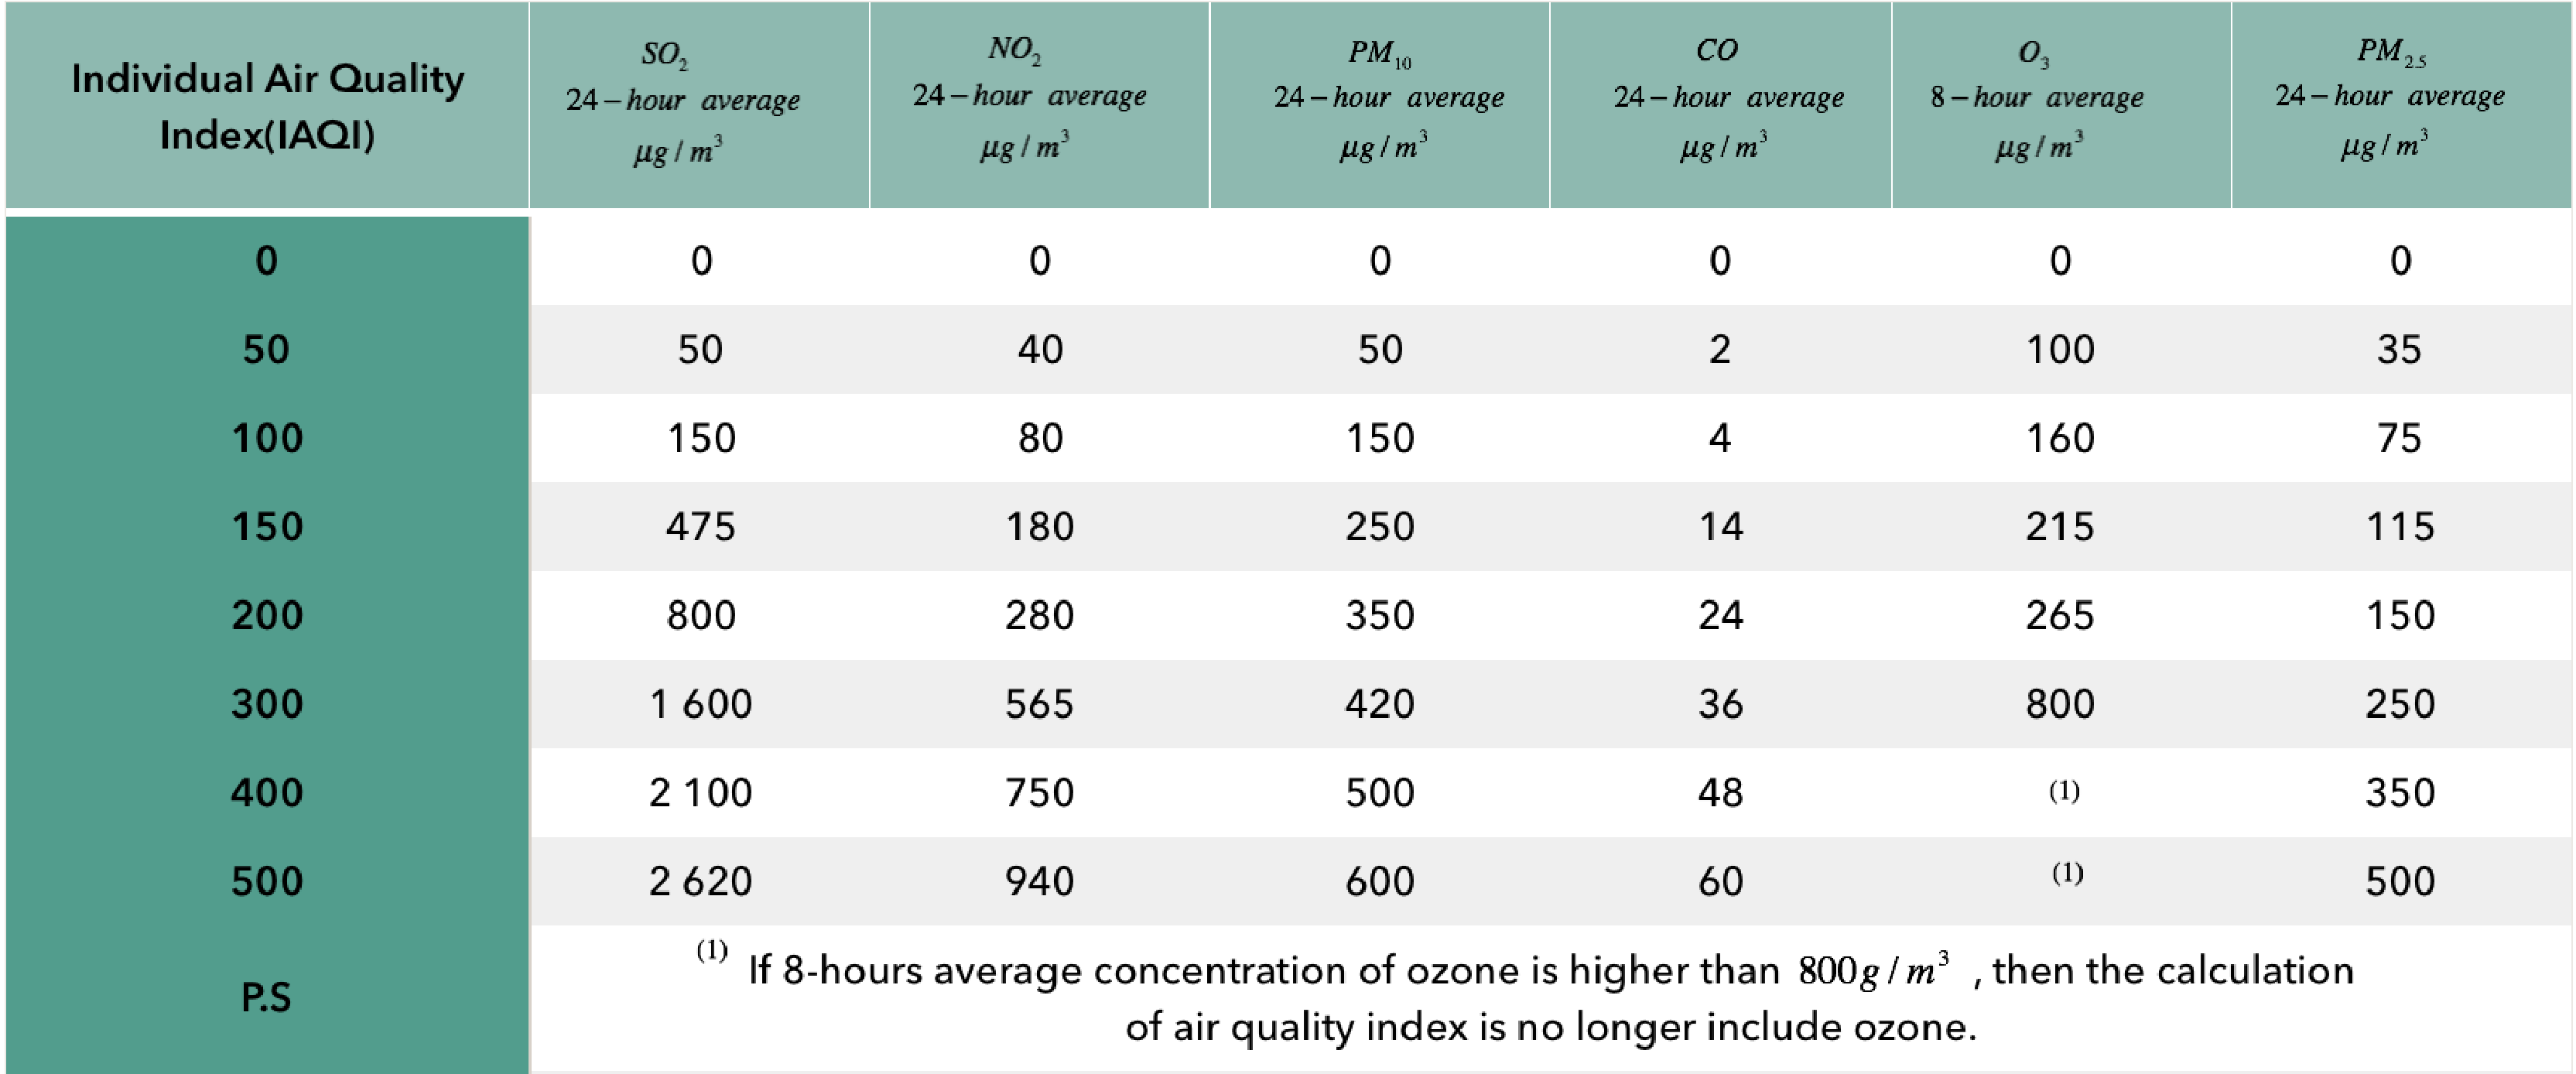
\includegraphics[width=16cm]{./Pic/AQItable.pdf}
\label{fig:graph}
\end{figure}

\paragraph {(2) Air Quality Index Calculation Method}
\textrm{\\}
%强制换行
\par Air quality index of pollutant item~$P$~is calculated according to equation(\ref{equ:IAQI}):
\begin{equation}
IAQI_{P}=\frac{IAQI_{Hi}-IAQI_{Lo}}{BP_{Hi}-BP_{Lo}}(C_{P}-BP_{Lo})+IAQI_{Lo}
\label{equ:IAQI} 
\end{equation}
Where:
\begin{itemize}
\item $IAQI_{P}$----Air quality index of pollutant item
\item $BP_{Hi}$----High value of pollutant concentration limit with~$CP$ in table(\ref{tab:AQI})
\item $BP_{Lo}$----Low value of pollutant concentration limit with~$CP$ in table(\ref{tab:AQI})
\item $IAQI_{Hi}$----Air quality index corresponding to ~$BP_{Hi}$ in table(\ref{tab:AQI})
\item $IAQI_{Lo}$----Air quality index corresponding to ~$BP_{Lo}$ in table(\ref{tab:AQI})
\end{itemize}



\subsubsection{Air Quality Index and Method for Determination of Primary Pollutant}
\paragraph {(1) Air Quality Index Calculation Method}
\textrm{\\}
\par Air quality index is calculating according to equation(\ref{equ:AQI}):
\begin{equation}
AQI=max\left \{{IAQI_{1},IAQI_{2},IAQI_{3},...,IAQI_{n}}  \right \}
\label{equ:AQI}
\end{equation}

Where:
\begin{itemize}
\item $IAQI$----Air quality index
\item $n$----Pollutant items
\end{itemize}

\paragraph {(2) Method for Determination of Primary Pollutant}
\textrm{\\}
\par When $AQI$ is greater than 50, the biggest pollutant of $IAQI$ is the primary pollutant. If the largest pollutant of $IAQI$ are two or more than two items, we set all of them as the primary pollutant.

\subsection{Data Capture}
\par In order to establish a reasonable evaluation index and make a reasonable assessment of the air quality changing trend in recent years, aiming at different time and spatial domain in Xi'an. We need to refer to some vital data from reasonable websites.
\par After searching data through surfing the Internet, we find that the \textbf{\emph{Xi'an environmental monitoring station}} \cite{RB} has authoritative data. In their website, we can not only obtain the historical data from 2010 to 2015, but also the independent data of each monitoring station distributed in Xi'an City. The following figure(\ref{fig:XianAQI}) is the screenshot of the website.
\begin{figure}[h]%[!hptb] !h意思是忽略美学标准,将照片固定到此位置;不会上下浮动% 支持格式eps, pdf, png, jpg
\centering %使得插入的照片居中显示
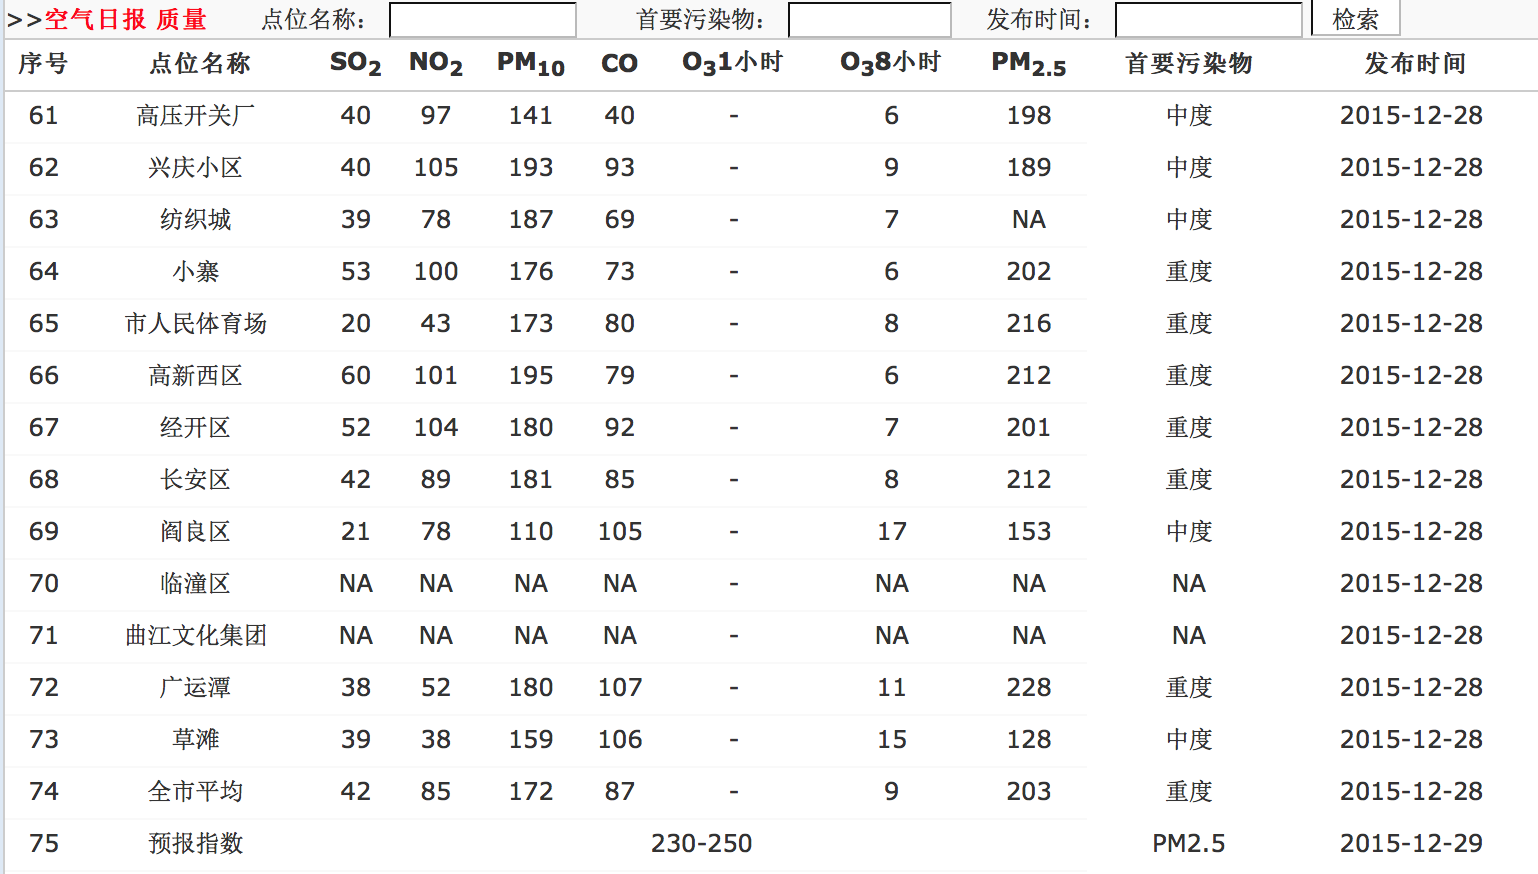
\includegraphics[width=0.8\textwidth]{./Pic/XianAQI.png}
% 图片标题
\caption{Air Quality Historical Data of Xi'an Partly(2010-2015)} 
\label{fig:XianAQI}  
\end{figure}
\par Obviously, we can not manually download such a huge data. Therefore, our team write a \textbf{\emph{web crawler}} program using \textbf{\emph{Python} }to automatically obtain all the historical data of the website.The following table(\ref{tab:webcrawler}) is the partly result of the web crawler fetching.

\begin{table}[htbp]
  \centering
  \caption{Data Acquired by Web Crawler}
    \begin{tabular}{ccccccccc}
    \toprule
    No.   & Location & SO2   & NO2   & PM10  & CO    & O3    & PM2.5 & Time \\
    \midrule
    1     & High Voltage Switch Factory & 59    & 112   & 115   & 27    & 18    & 137   & 2016-1-1 \\
    2     & Xingqing Garden & 61    & 121   & 140   & 94    & 14    & 139   & 2016-1-1 \\
    3     & Textile City & 44    & 72    & 132   & 75    & 19    & 220   & 2016-1-1 \\
    4     & Xiaozhai & 53    & 108   & 126   & 84    & 14    & 129   & 2016-1-1 \\
    5     & Gym   & 27    & 57    & 148   & 91    & 14    & 196   & 2016-1-1 \\
    6     & High-tech Development West Zone & 59    & 101   & 165   & 92    & 21    & 190   & 2016-1-1 \\
    7     & Economic Development Zone & 54    & 120   & 185   & 103   & 20    & 212   & 2016-1-1 \\
    8     & Changan & 52    & 105   & 119   & 101   & 26    & 127   & 2016-1-1 \\
    9     & Yanliang & NA    & NA    & NA    & NA    & NA    & NA    & 2016-1-1 \\
    10    & Lintong & 57    & 79    & 142   & 91    & 17    & 166   & 2016-1-1 \\
    11    & Qujiang & 15    & 55    & 168   & 30    & 7     & NA    & 2016-1-1 \\
    12    & Guangyuntan & 56    & 58    & 168   & 113   & 14    & 227   & 2016-1-1 \\
    13    & Caotan & 72    & 63    & 181   & 116   & 31    & 172   & 2016-1-1 \\
    \bottomrule
    \end{tabular}%
  \label{tab:webcrawler}%
\end{table}%



\section{Problem \uppercase\expandafter{\romannumeral1}}
\subsection{Time Analysis Model Based on Discrete Wavelet Transform}

\par In numerical analysis and functional analysis, a discrete wavelet transform (DWT) is any wavelet transform for which the wavelets are discretely sampled. As with other wavelet transforms, a key advantage it has over Fourier transforms is temporal resolution: it captures both frequency and location information (location in time).
\par By coincidence, in the temporal variation analysis of air quality, the data we have obtained is discrete, so we will use the method based on discrete wavelet transform to discover the trend of AQI.

\paragraph{One level of the transform}
\textrm{\\}
    \par The DWT of a signal ~$x$~ is calculated by passing it through a series of filters. First the samples are passed through a low pass filter with impulse response ~$g$~ resulting in a convolution of the two:
    \begin{equation}
    y[n] = (x \times g)[n] = \sum\limits_{k =  - \infty }^\infty  {x[k] g[n - k]} 
    \end{equation}
    \par The signal is also decomposed simultaneously using a high-pass filter~$h$~. The outputs giving the detail coefficients (from the high-pass filter) and approximation coefficients (from the low-pass). It is important that the two filters are related to each other and they are known as a quadrature mirror filter.
    \begin{figure}[h]%[!hptb] !h意思是忽略美学标准,将照片固定到此位置;不会上下浮动% 支持格式eps, pdf, png, jpg
    \centering %使得插入的照片居中显示
    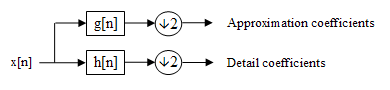
\includegraphics[width=0.8\textwidth]{./Pic/WaveletsDWT.png}
    % 图片标题
    \caption{Block diagram of filter analysis} 
    \label{fig:WaveletsDWT}  
    \end{figure}
    \par However, since half the frequencies of the signal have now been removed, half the samples can be discarded according to Nyquist‘s rule. The filter outputs are then subsampled by 2. In the next two formulas, the notation is the opposite: g- denotes high pass and h- low pass as is Mallat's and the common notation:

    \begin{equation}
    y_{\mathrm{low}} [n] = \sum\limits_{k =  - \infty }^\infty  {x[k] h[2 n - k]} 
    \end{equation}

    \begin{equation}
    y_{\mathrm{high}} [n] = \sum\limits_{k =  - \infty }^\infty  {x[k] g[2 n - k]} 
    \end{equation}
    \par This decomposition has halved the time resolution since only half of each filter output characterises the signal. However, each output has half the frequency band of the input so the frequency resolution has been doubled.
    \par With the subsampling operator $\downarrow$
    \begin{equation}
    (y \downarrow k)[n] = y[kn] 
    \end{equation}
    \par the above summation can be written more concisely.

    \begin{equation}
    y_{\mathrm{low}} = (x\times g)\downarrow 2 
    \end{equation}

    \begin{equation}
    y_{\mathrm{high}} = (x\times h)\downarrow 2 
    \end{equation}
    \par However computing a complete convolution ~$x\times g$ with subsequent downsampling would waste computation time.

    \par The Lifting scheme is an optimization where these two computations are interleaved.



\paragraph{Cascading and Filter banks}
\textrm{\\}
\par This decomposition is repeated to further increase the frequency resolution and the approximation coefficients decomposed with high and low pass filters and then down-sampled. This is represented as a binary tree with nodes representing a sub-space with a different time-frequency localisation. The tree is known as a filter bank.

    \begin{figure}[h]%[!hptb] !h意思是忽略美学标准,将照片固定到此位置;不会上下浮动% 支持格式eps, pdf, png, jpg
    \centering %使得插入的照片居中显示
    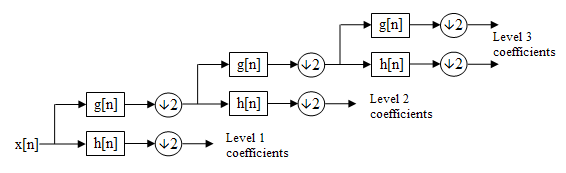
\includegraphics[width=0.8\textwidth]{./Pic/WaveletsFilterBank.png}
    % 图片标题
    \caption{A $3$ level filter bank} 
    \label{fig:WaveletsFilterBank}  
    \end{figure}
\par At each level in the above diagram the signal is decomposed into low and high frequencies. Due to the decomposition process the input signal must be a multiple of $2^n$ where $n$ is the number of levels.


\paragraph{Relationship to the Mother Wavelet}
\textrm{\\}
\par The filterbank implementation of wavelets can be interpreted as computing the wavelet coefficients of a discrete set of child wavelets for a given mother wavelet $\psi(t)$. In the case of the discrete wavelet transform, the mother wavelet is shifted and scaled by powers of two
\begin{equation}
 \psi_{j,k}(t)= \frac{1}{\sqrt{2^j}} \psi \left( \frac{t - k2^j}{2^j} \right) 
\end{equation}

\par where $j$ is the scale parameter and $k$ is the shift parameter, both which are integers.

\par Recall that the wavelet coefficient $\gamma$ of a signal $x(t)$ is the projection of $x(t)$ onto a wavelet, and let $x(t)$ be a signal of length $2^N$. In the case of a child wavelet in the discrete family above,
\begin{equation}
 \gamma_{jk}=\int_{-\infty}^{\infty}x(t)  
 \frac{1}{\sqrt{2^j}}\psi\left(\frac{t-k2^j}{2^j} \right)dt 
\end{equation}

\par Now fix $j$ at a particular scale, so that  $\gamma_{jk}$  is a function of $k$ only. In light of the above equation, $\gamma_{jk}$ can be viewed as a convolution of $x(t)$ with a dilated, reflected, and normalized version of the mother wavelet, $h(t) = \frac{1}{\sqrt{2^j}}\psi\left(\frac{-t}{2^j}\right)$, sampled at the points $1, 2^j, 2^{2j}, ..., 2^{N}$. But this is precisely what the detail coefficients give at level $j$ of the discrete wavelet transform. Therefore, for an appropriate choice of $h[n]$ and $g[n]$, the detail coefficients of the filter bank correspond exactly to a wavelet coefficient of a discrete set of child wavelets for a given mother wavelet $\psi(t)$.
\par In this problem, we use \textbf{\emph{daubechies(dbN)}} function ($N$ takes $6$) as the mother wavelet, and decompose $4$ layers. Finally, get the following results:

\begin{figure}[h]
  \centering %使得插入的照片居中显示
  \begin{minipage}[t]{.49\linewidth}
   % \framebox{Text}
  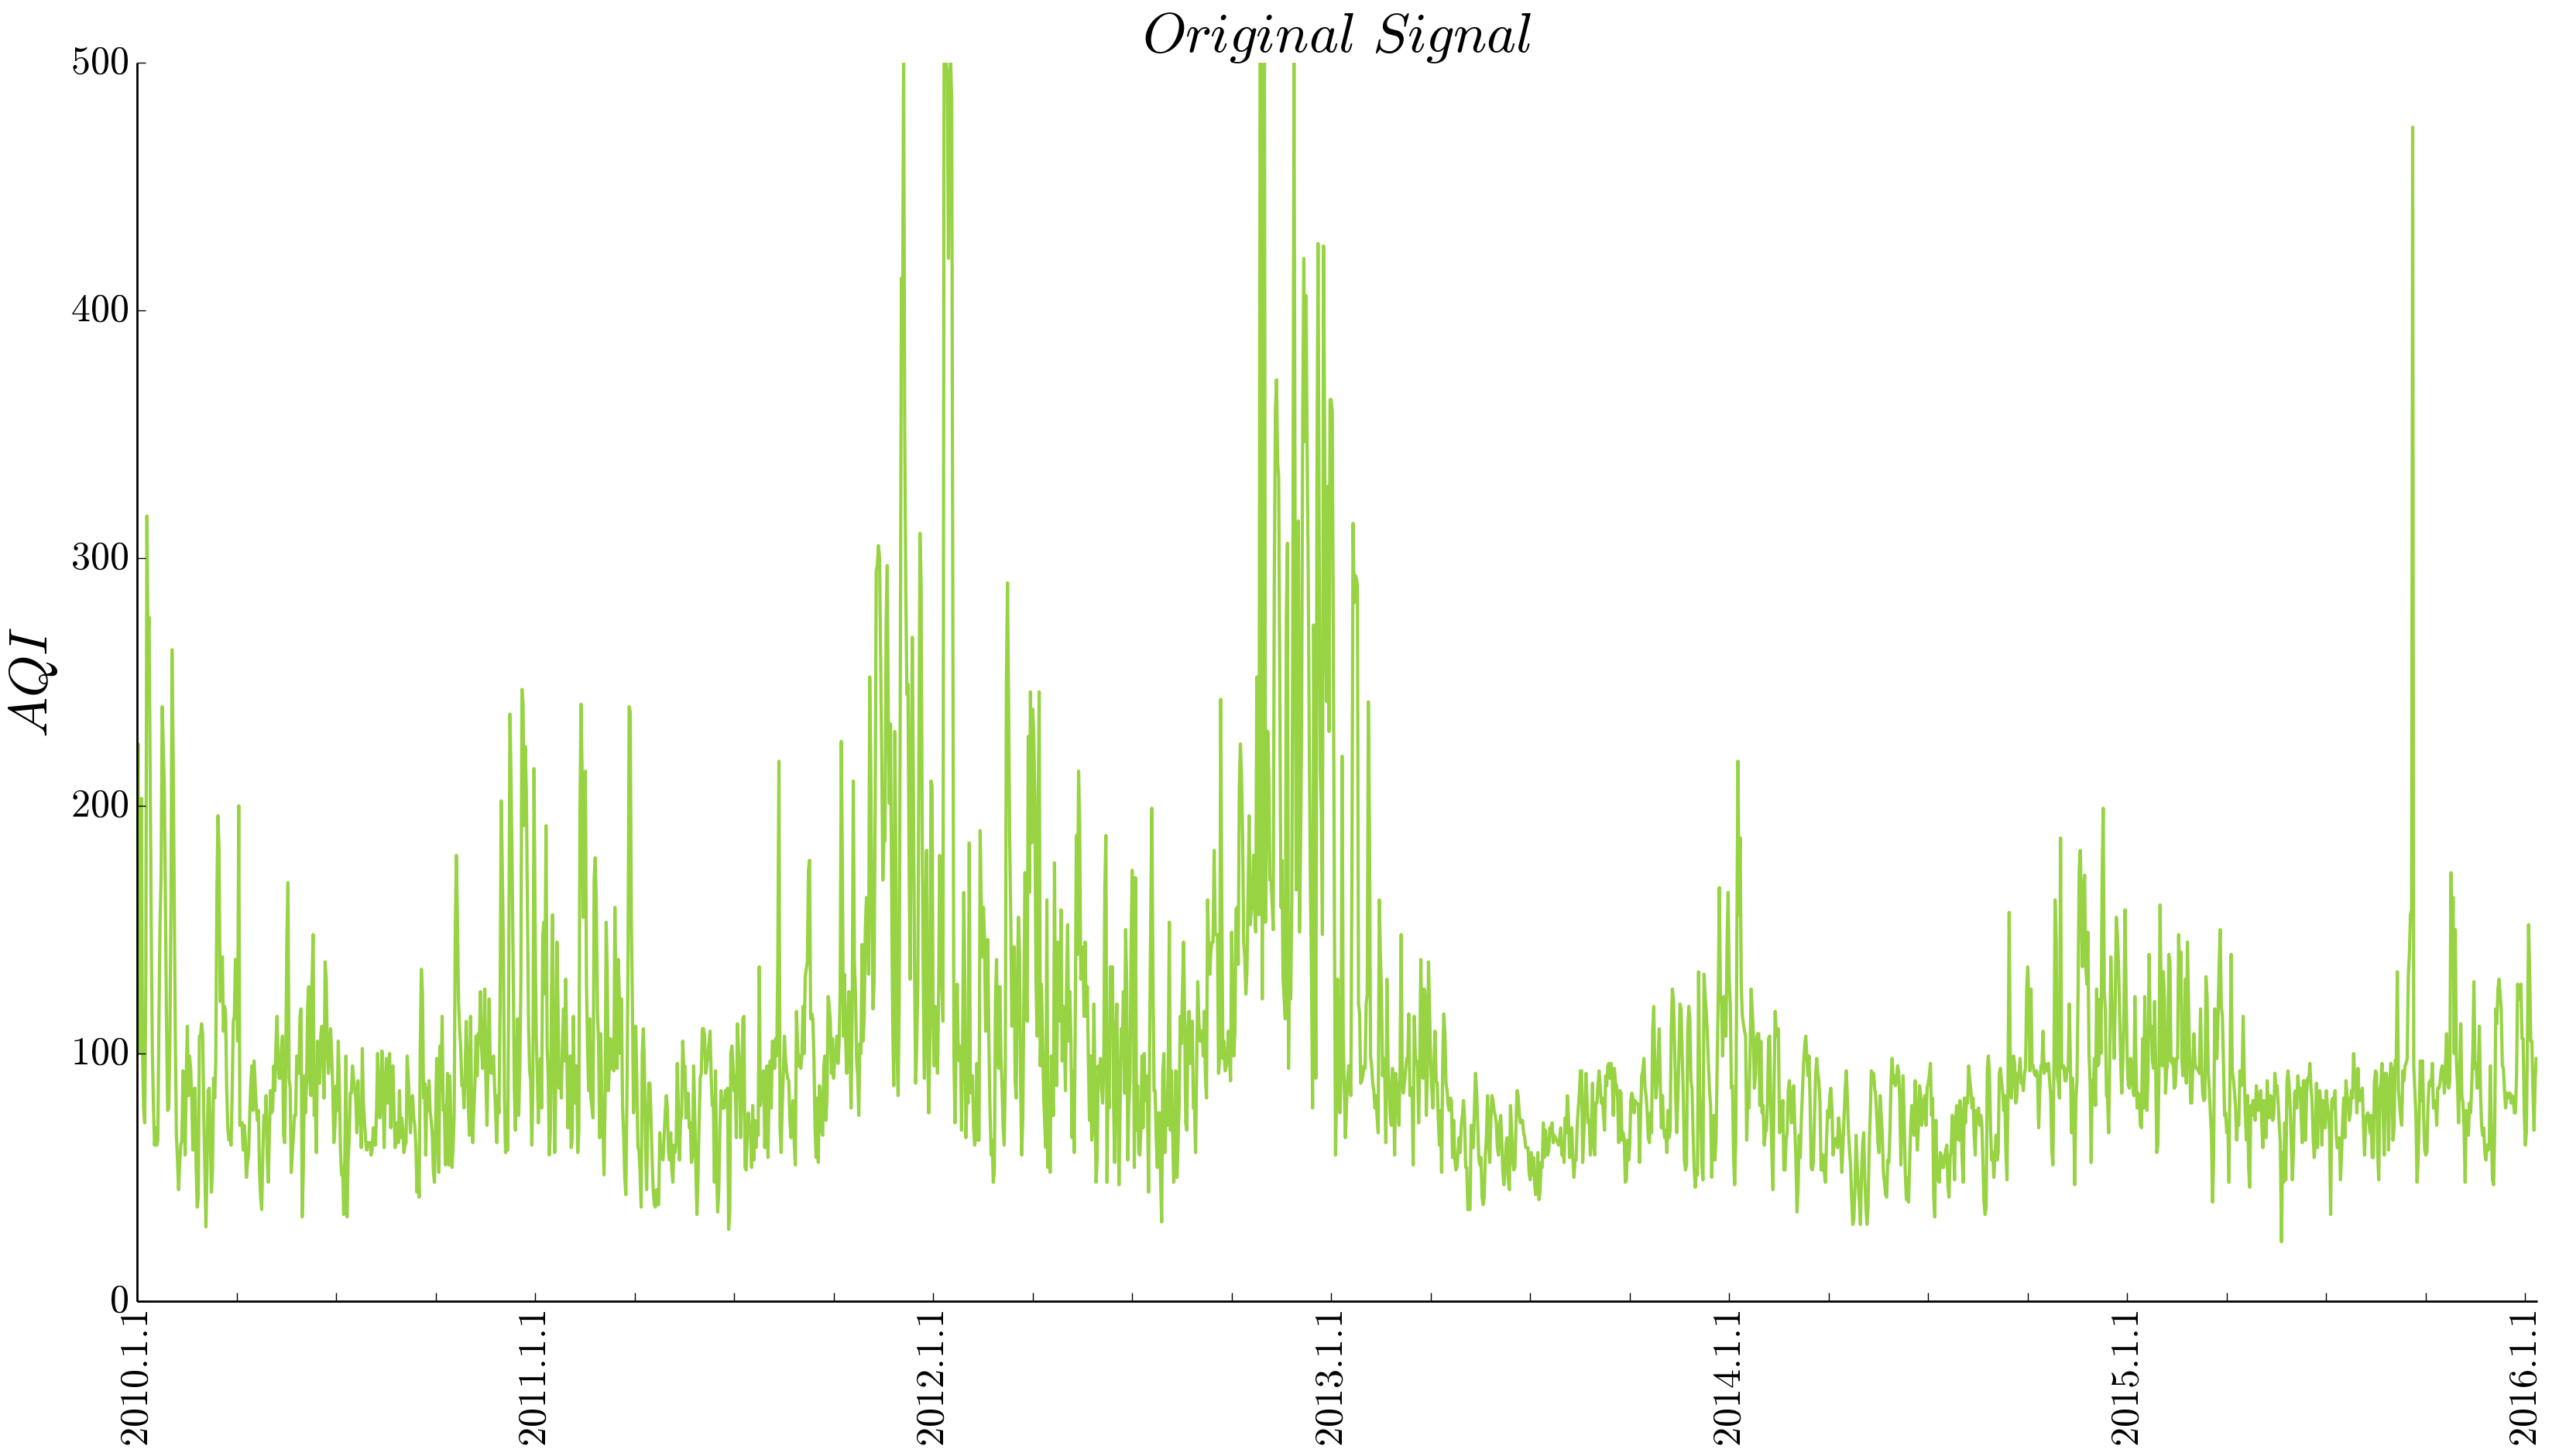
\includegraphics[width=1\textwidth]{./Pic/NO1/Trsorigin.png}
  \caption{the Original Data of AQI(2010-2015)}
  \label{fig:od}
  \end{minipage}
  \begin{minipage}[t]{.49\linewidth}
  
  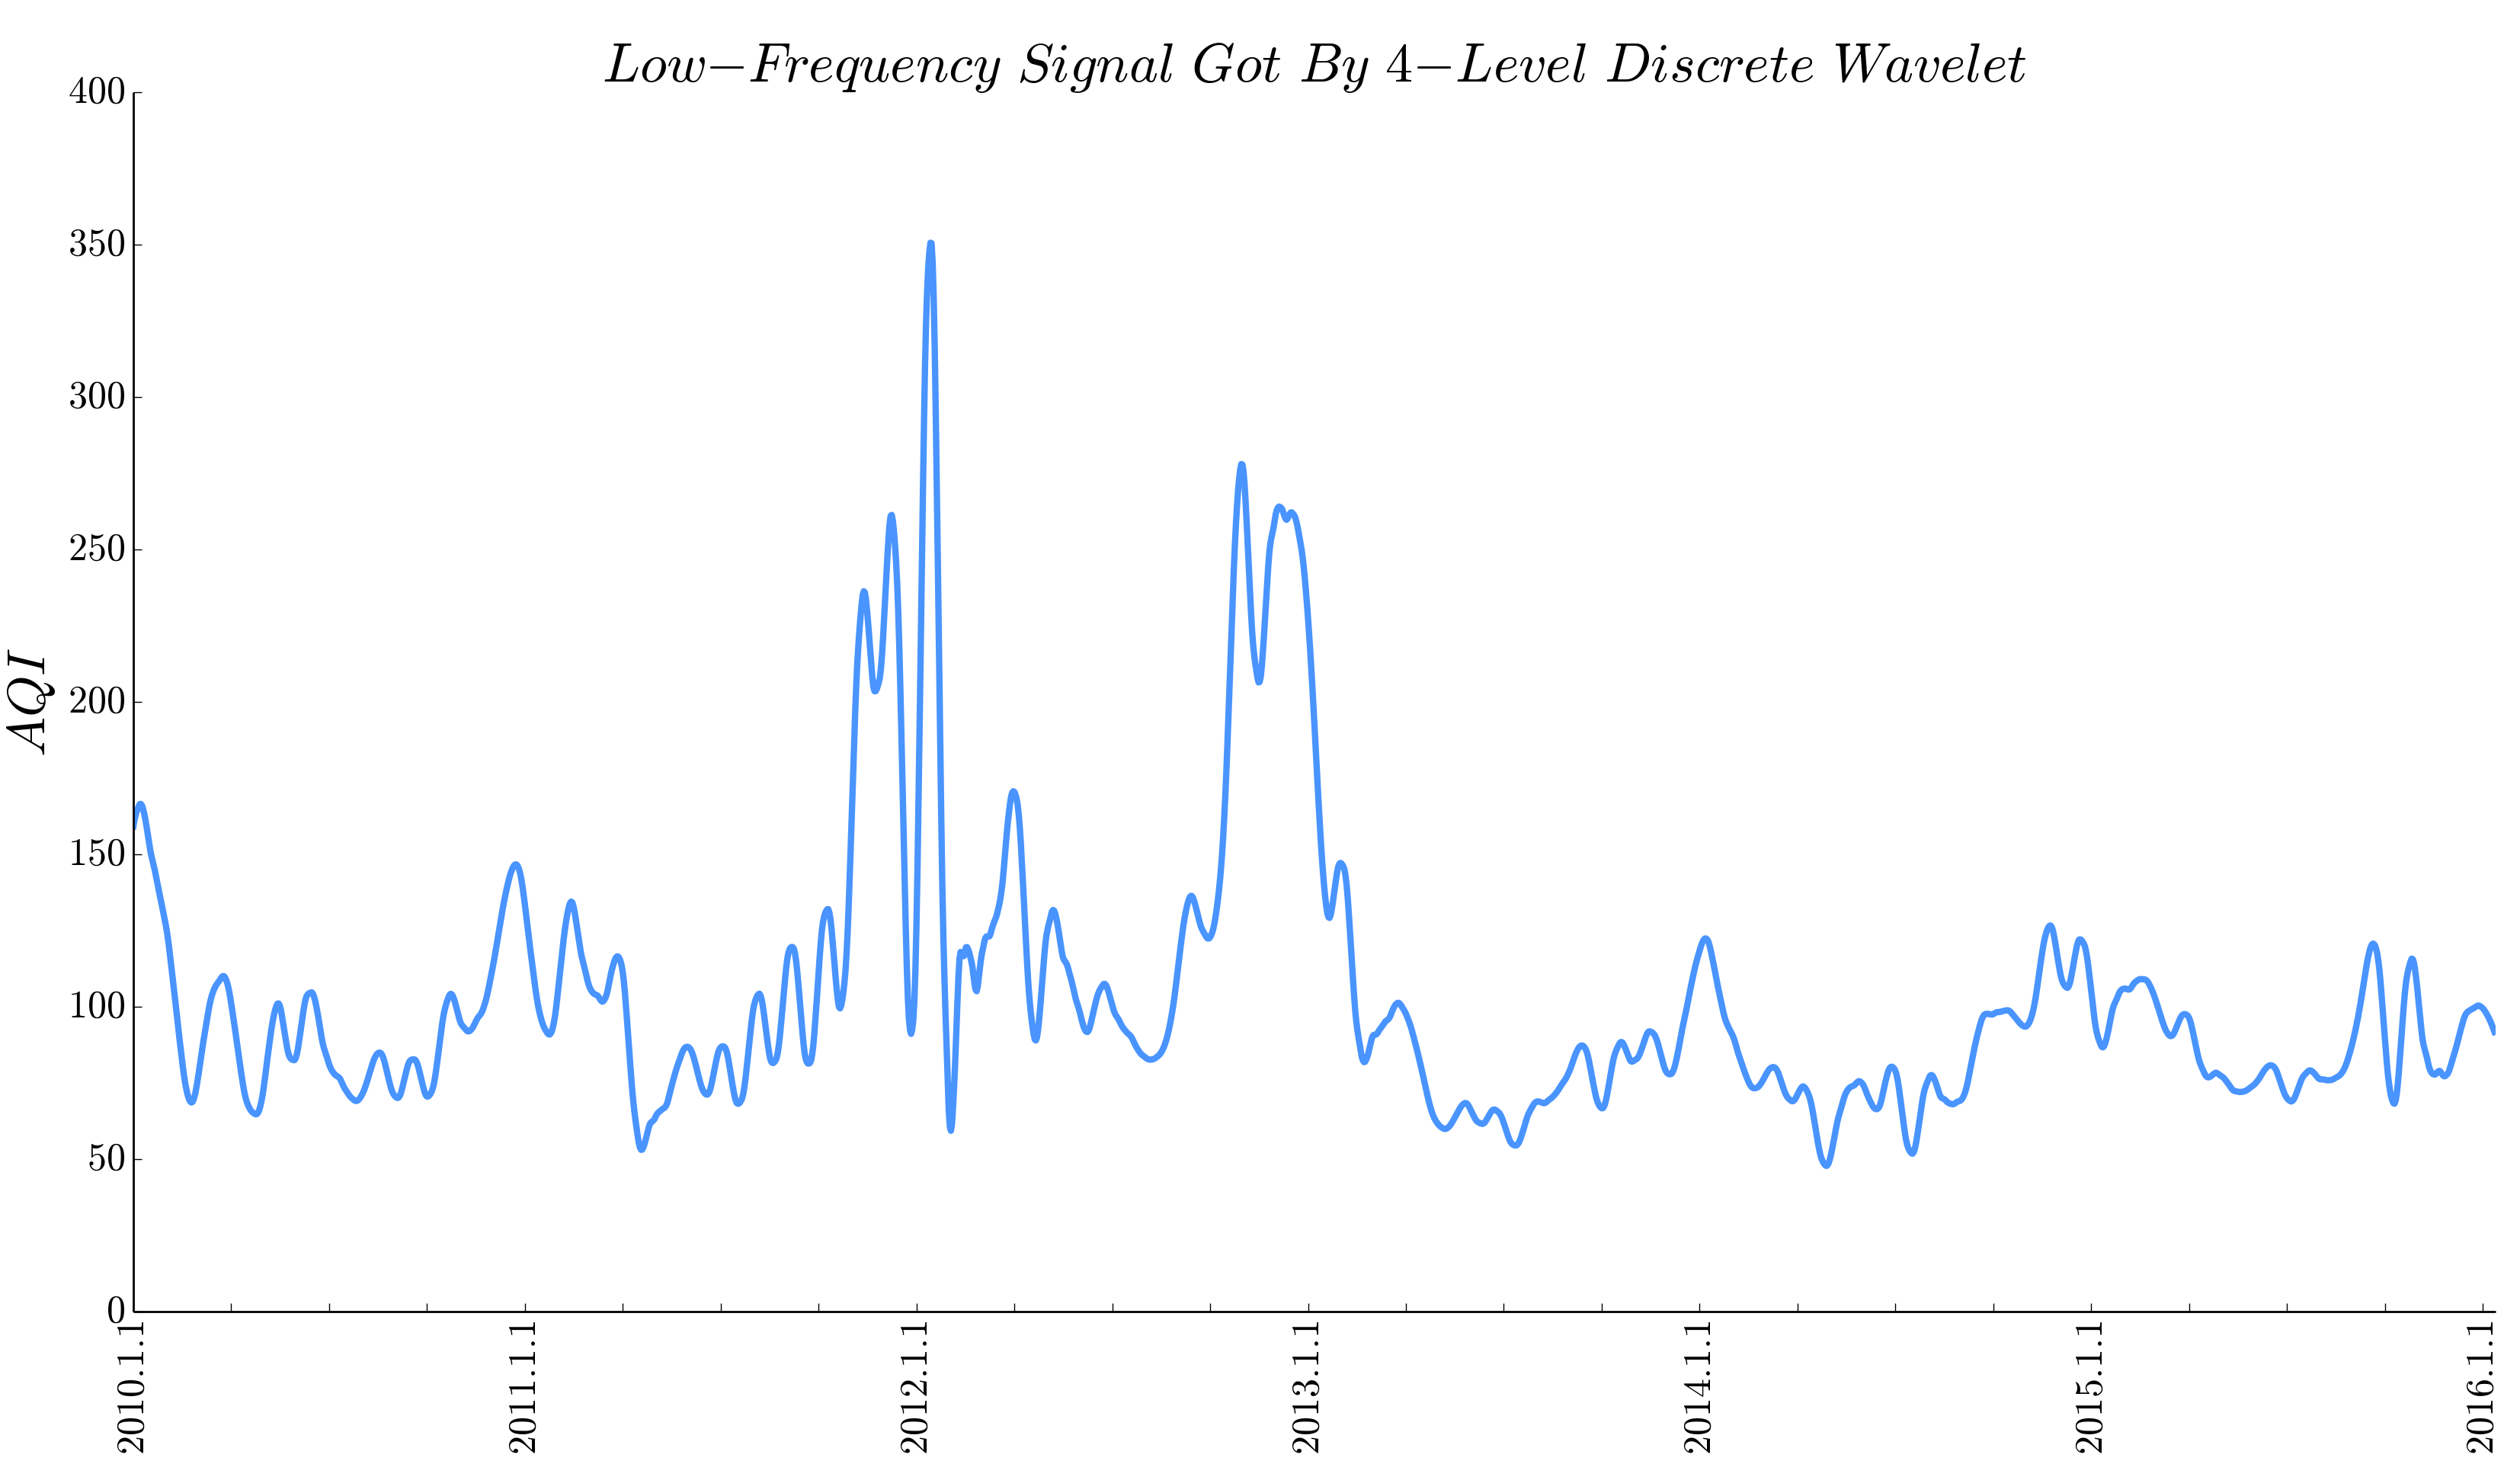
\includegraphics[width=1\textwidth]{./Pic/NO1/Trslowf.png}
  %\framebox{Text}
  \caption{Low-frequency Signal got by 4-level Discrete Wavelet}
  \label{fig:4-ld}
  \end{minipage}
\end{figure}



\par The figure(\ref{fig:od}) is the original data.After processing the data by 4-level $db6$ function, the result is shown in figure(\ref{fig:4-ld}).We can observe the change trend of the smooth curve approximately.
\par In order to be able to clearly predict the trend of air quality, we have reprocessed the data, and redraw the figure.Taking advantage of \textbf{\emph{Python}}, we divide the curve into 4 distinct time parts, and each part has a different color representing different season.
\begin{figure}[h]%[!hptb] !h意思是忽略美学标准,将照片固定到此位置;不会上下浮动% 支持格式eps, pdf, png, jpg
\centering %使得插入的照片居中显示
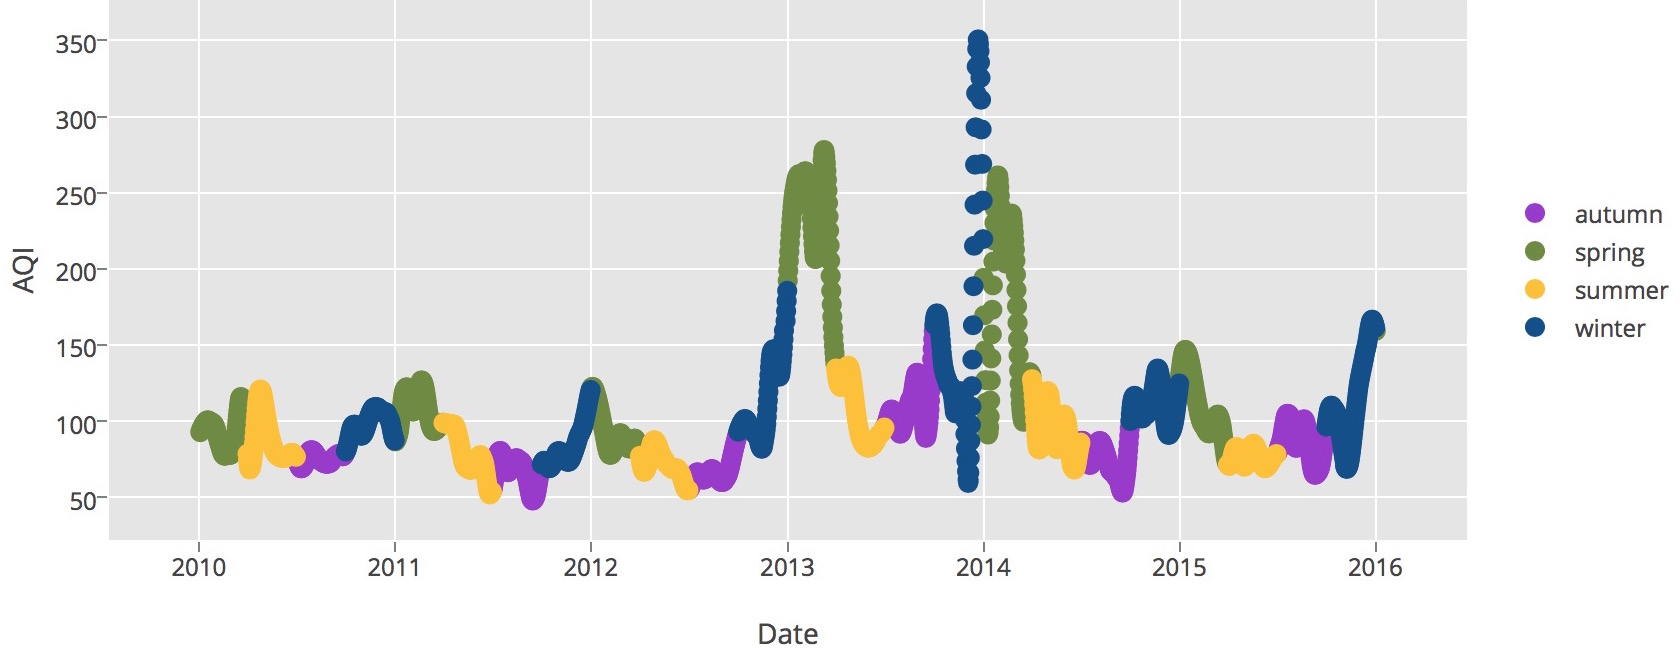
\includegraphics[width=0.8\textwidth]{./Pic/NO1/Trspart.jpg}
% 图片标题
\caption{the Figure afer Tranforming} 
\label{fig:Trspart}  
\end{figure}

\par From the figure(\ref{fig:Trspart}), we can see. the periodic variation of AQI is very obvious. AQI index is on the crest in spring (marked in green) and winter (marked in blue), significantly higher than in summer (marked in yellow) and autumn (marked in purple). From this figure, we can make a reasonable guess,  the periodic variation of AQI changes is seasonal. Winter and spring are the worst season in Xi'an, especially in December and January.


\subsection{Spatial Analysis Model Based on Discrete Wavelet Transform}
\par Using the above method, we analyze the spatial distribution of AQI.The figure(\ref{fig:3d}) is the result we obtain. In order to let the result visualization, we use the \textbf{\emph{Python}} to draw a 3-D map as follows.

\begin{figure}[h]%[!hptb] !h意思是忽略美学标准,将照片固定到此位置;不会上下浮动% 支持格式eps, pdf, png, jpg
\centering %使得插入的照片居中显示
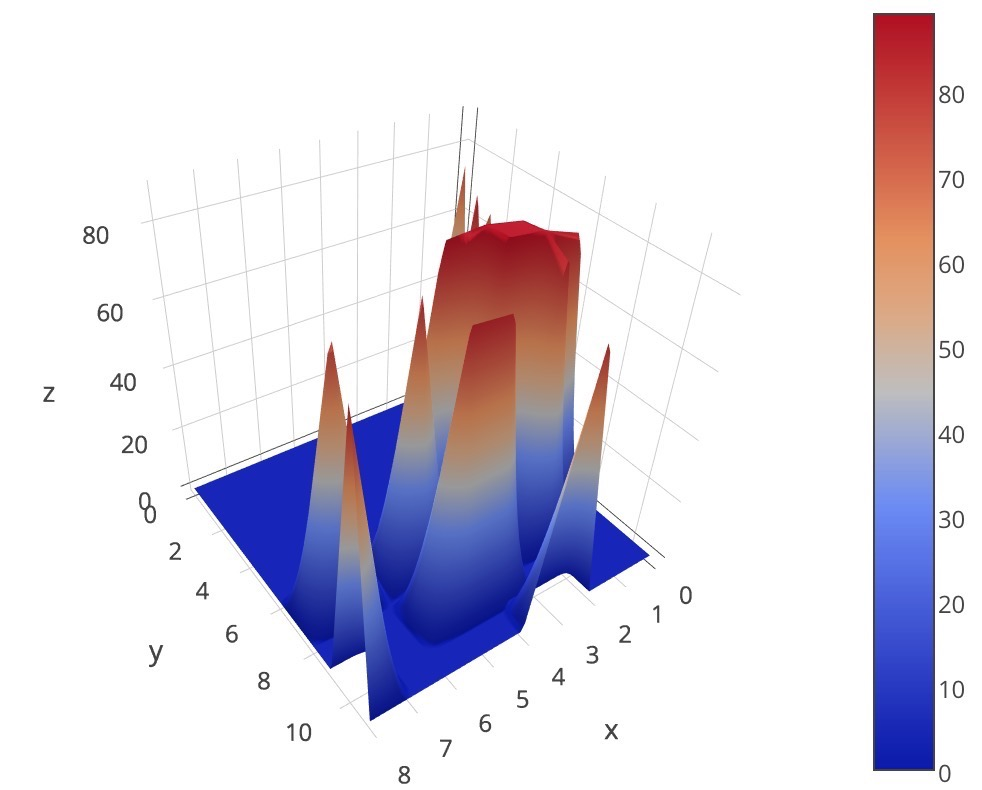
\includegraphics[width=0.50\textwidth]{./Pic/3d.jpg}
% 图片标题
\caption{the Territorial Classification}
\label{fig:3d}       % 给图片一个标签便于交叉引用
\end{figure}
\par In the figure(\ref{fig:3d}), the ~$X$~ axis represents the east and west direction, the ~$Y$~ asis represents the north and south direction, the ~$Z$~ axis represents the air pollution index.
\par From the figure, we can see, in the Central and Eastern Xi'an, air pollution is serious, the AQI is very high. The West and the surrounding areas of Xi'an, the air is better than the other areas, the index is low. The most polluted areas are Economic Development Area and the High Voltage Switch Factory. The lightest polluted area is Bayuntan. Overall air pollution in various regions of Xi'an city is slightly different.


\section{Problem \uppercase\expandafter{\romannumeral2}}

\par Through the analysis of the problem  \uppercase\expandafter{\romannumeral1}, we have obtained the variation trend of AQI with time and space. Referring to related knowledge and documentation, we come to the conclusion that the main factors mainly include two categories:emission of pollution sources and the weather.
\subsection{Emission of pollution}
\par An emission factor is a representative value that relates the quantity of a pollutant released to the atmosphere with an activity associated with the release of that pollutant. These factors are usually expressed as the weight of pollutant divided by a unit weight, volume, distance, or duration of the activity emitting the pollutant. Such factors facilitate estimation of emissions from various sources of air pollution. In most cases, these factors are simply averages of all available data of acceptable quality, and are generally assumed to be representative of long-term averages for all facilities in the source category. The emission factor is used to calculate the total emission from a source as an input for the emission inventory.
\paragraph{Cluster Analysis Model of Emission Factor}
\textrm{\\}
\par The difference of pollution source emission is mainly from space. We have to analyse the pollution sources in different regions and make comparison. As the observation point is too much to analyse, therefore, we use the method of cluster analysis to process the data, dividing them into 5 classifications.
\paragraph{Definition}
\textrm{\\}
\par Cluster analysis or clustering is the task of grouping a set of objects in such a way that objects in the same group (called a cluster) are more similar (in some sense or another) to each other than to those in other groups (clusters). It is a main task of exploratory data mining, and a common technique for statistical data analysis, used in many fields, including machine learning, pattern recognition, image analysis, information retrieval, and bioinformatics.
\paragraph{Cluster Analysis Process}
\textrm{\\}
\par Above is the basic definition of the clustering method, the following is the specific process of data clustering.
\begin{enumerate}%[(1)]
\renewcommand{\labelenumi}{(\theenumi)}
    \item Selecting clustering method. In this paper, we use the Ward method which is integrated in SPSS \cite{RC} software, and use \textbf{\emph{Eucidean Distance}} to measure distance. 
    \item Calculate the distance between $n$ samples, and obtain the distance matrix $D^(0)$.
    \item At first, $n$ samples constitute n classes by themselves(the first step:$i=1$), and the $i^th$ class is $G_i={X_{(i)}}~(i=1,2,3,...,n)$. At this time, the distance between classes is the distance between samples ($D^{(1)}=D^W$). And then perform the next $4^th$ and $5^th$ step of the sample.
    \item The next step is amalgamating the two classes with the smallest distance into a new class. The total number of classes at this time is reduced 1 class, ~$k=n-i+1$.
    \item Calculate the distance between the new class and the other classes, and get a new distance matrix ~$D^{(1)}$. If the total number $k$ of the merged class is more than 1, repeat steps 4 and 5 until the number of classes is 1, and then go to step 6.
    \item Draw the diagram of pedigree clustering, and decide the number of class and the members the of each class.
\end{enumerate}



\begin{figure}[h]
  \centering %使得插入的照片居中显示
  \begin{minipage}[t]{.4\linewidth}
   % \framebox{Text}
\centering %使得插入的照片居中显示
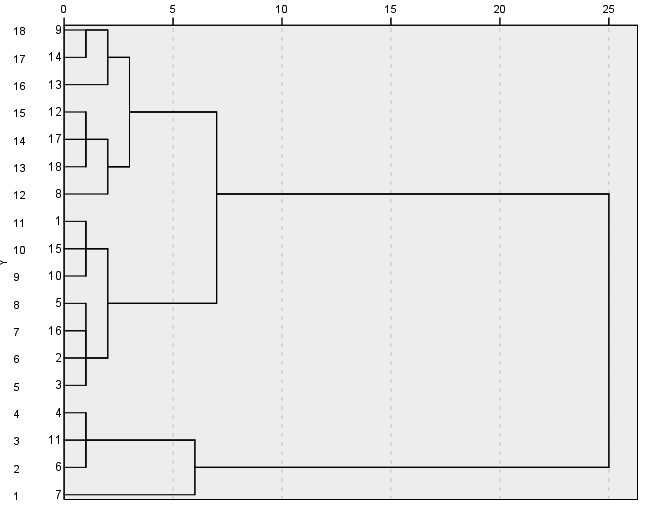
\includegraphics[width=1.0\textwidth]{./Pic/5class1.png}
% 图片标题
\caption{the Territorial Classification}
\label{fig:5class1}  
  \end{minipage}
  \begin{minipage}[t]{.4\linewidth}
  
  \centering %使得插入的照片居中显示
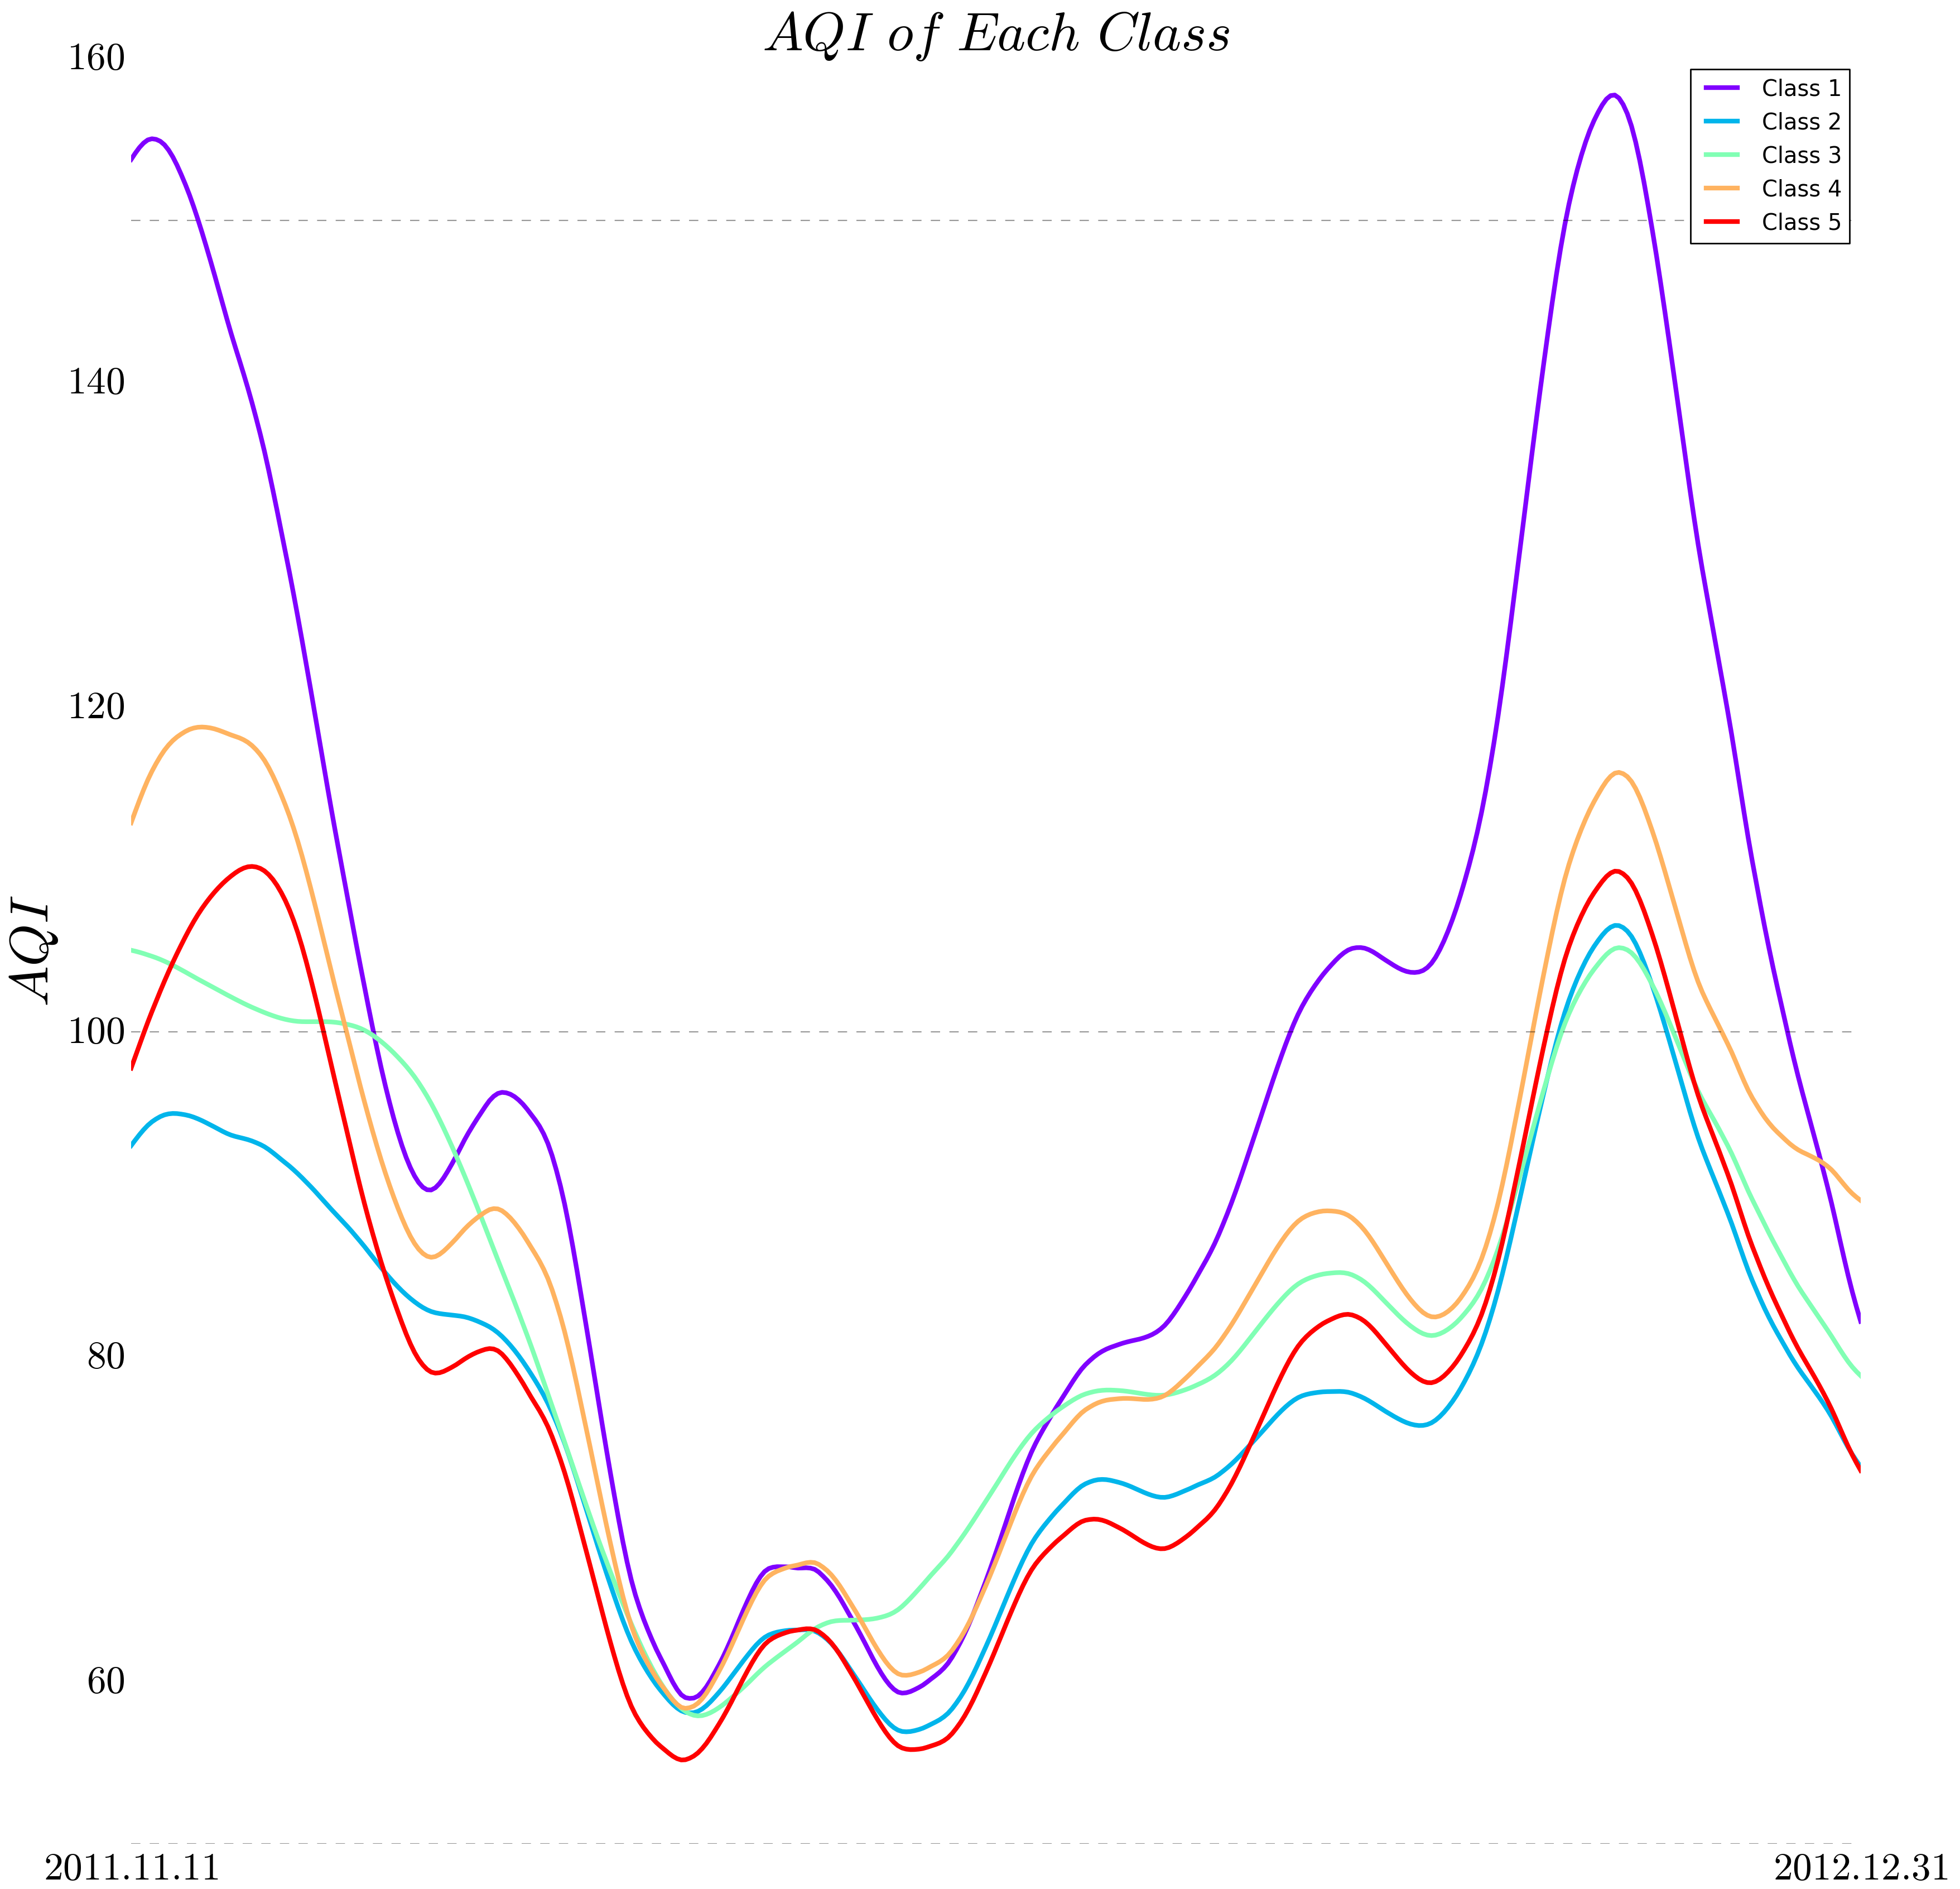
\includegraphics[width=1.0\textwidth]{./Pic/5class2.png}
% 图片标题
\caption{AQI of Each Class}
\label{fig:5class2}  
  \end{minipage}
\end{figure}


\begin{table}[h]
  \centering
  \caption{Classes of Regions in Xi'an}
    \begin{tabular}{ccccc}
    \toprule
    1     & 2     & 3     & 4     & 5 \\
    \midrule
    Factory & Ganting & Caotan & Doumen & Guangyuntan \\
    Xingqing & languan &       & Lintong & luxiang \\
    Textile & Bayunta &       & Yanliang & Qujiang \\
    hightech &       &       & Changan &  \\
    economicdevelopment &       &       &       &  \\
    Gym   &       &       &       &  \\
    Xiaozhai &       &       &       &  \\
    \bottomrule
    \end{tabular}%
  \label{tab:5class}%
\end{table}%



\par The figure above is shown the variation trend of AQI after cluster analysis.
\subsection{Weather}
\par To analyze the influence factors of air condition, we have to consider the impact of climate on it. There have lots of impact factors included in climate. After analysing(compare each curve of the factors with mothly AQI), we fully convince that the following three factors are the vitalest.



\begin{figure}[h]
  \centering %使得插入的照片居中显示
  \begin{minipage}[t]{.4\linewidth}
   % \framebox{Text}
  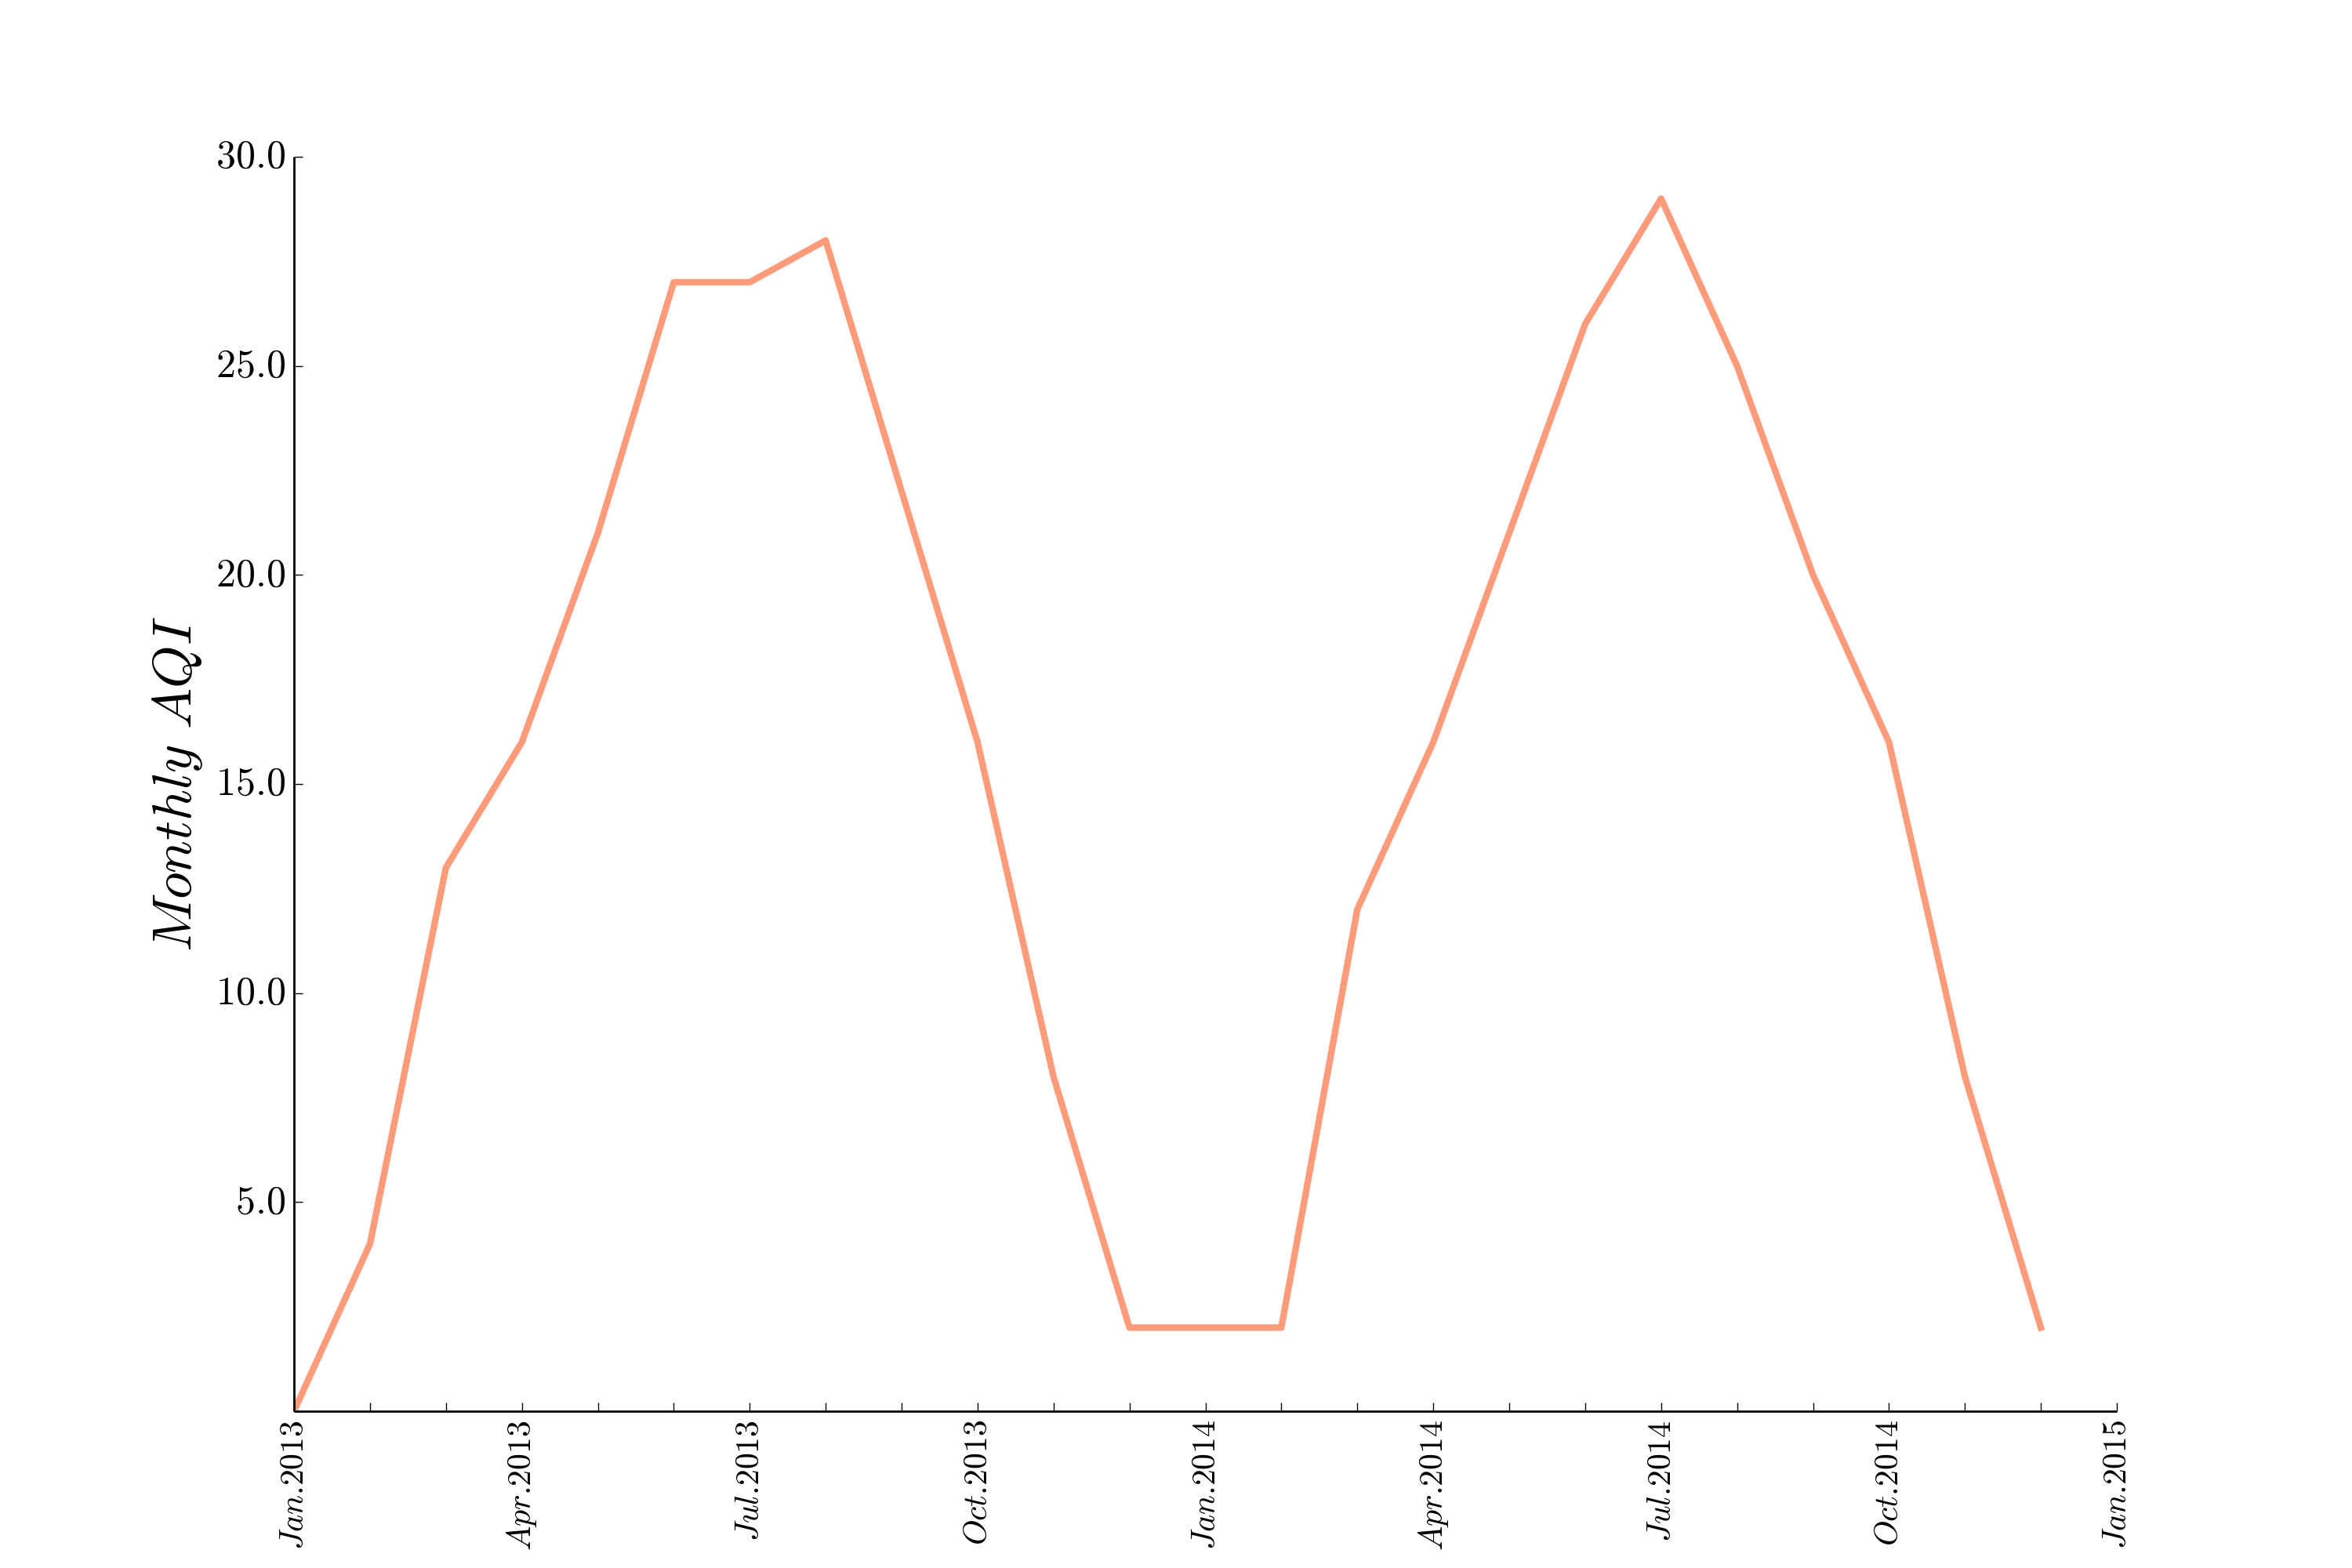
\includegraphics[width=1\textwidth]{./Pic/mothlyAQI.png}
  \caption{AQI Monthly(2013-2014)}
  \label{fig:mothlyAQI}
  \end{minipage}
  \begin{minipage}[t]{.4\linewidth}
  
  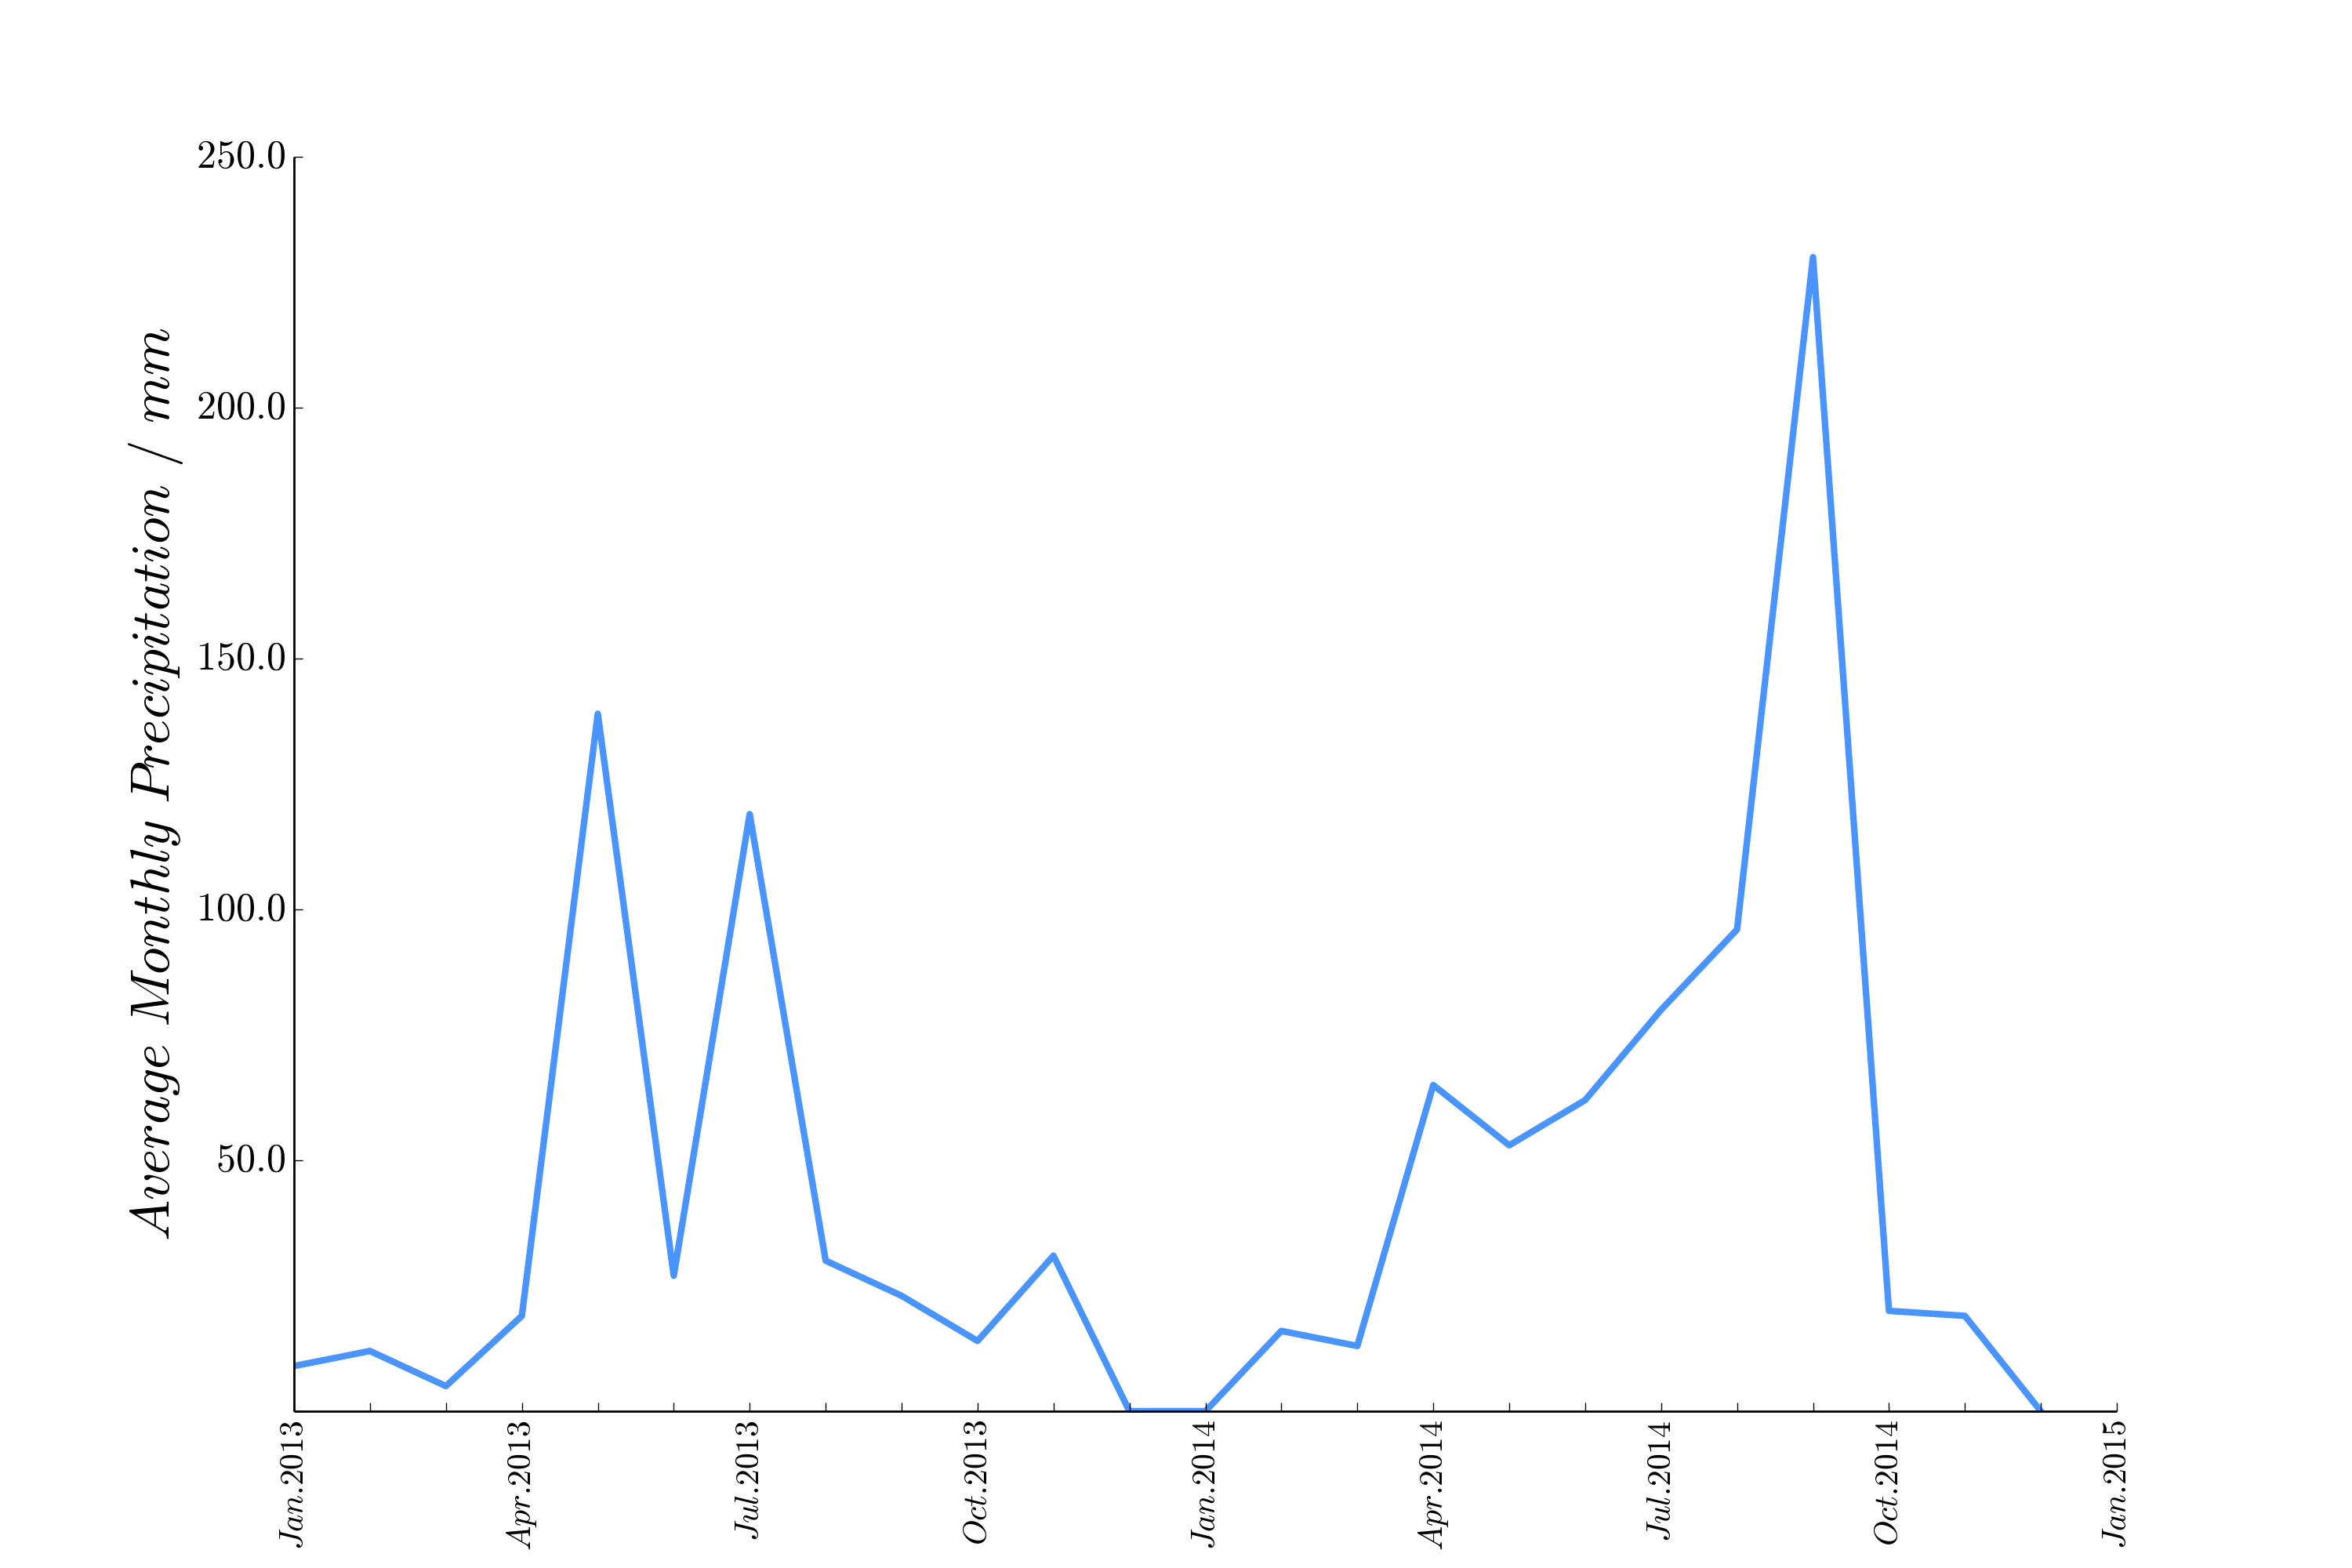
\includegraphics[width=1\textwidth]{./Pic/js.png}
  %\framebox{Text}
  \caption{Average Precipitation Monthly(2013-2014)}
  \label{fig:js}
  \end{minipage}
\end{figure}



\begin{figure}[h]
  \centering %使得插入的照片居中显示
  \begin{minipage}[t]{.4\linewidth}
   % \framebox{Text}
  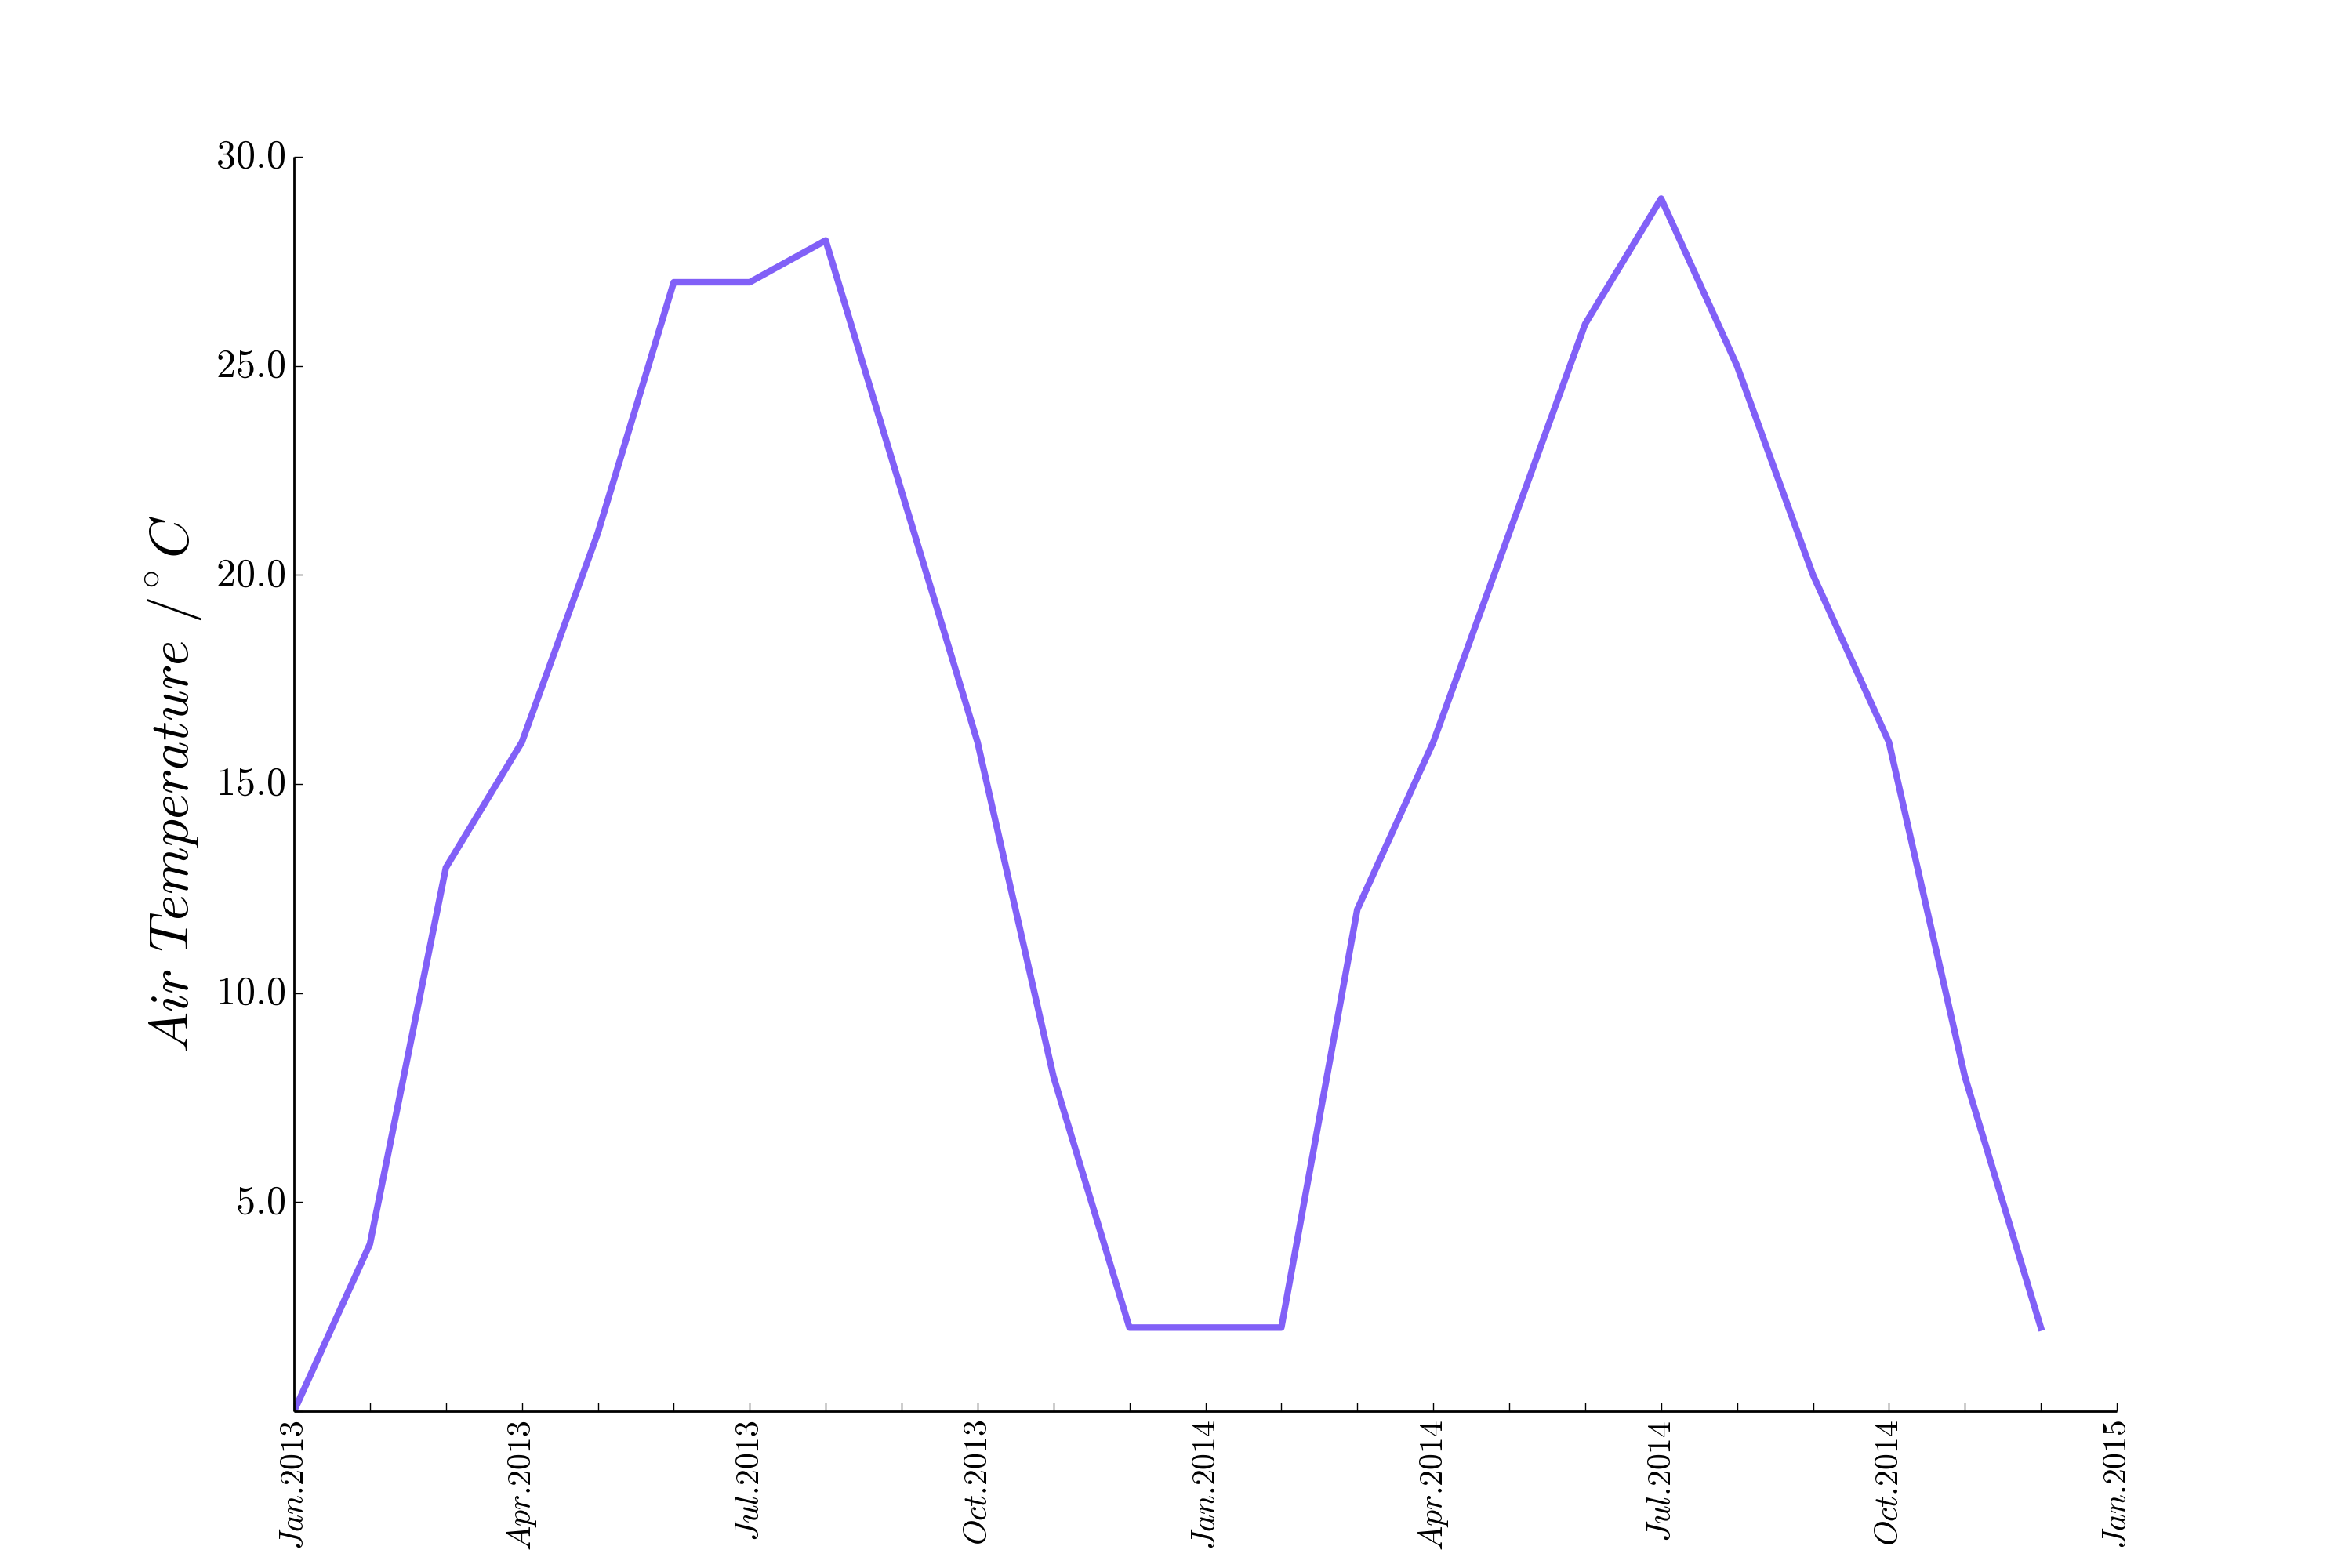
\includegraphics[width=1\textwidth]{./Pic/tp.png}
  \caption{Average Temperature Monthly(2013-2014)}
  \label{fig:tp}
  \end{minipage}
  \begin{minipage}[t]{.4\linewidth}
  
  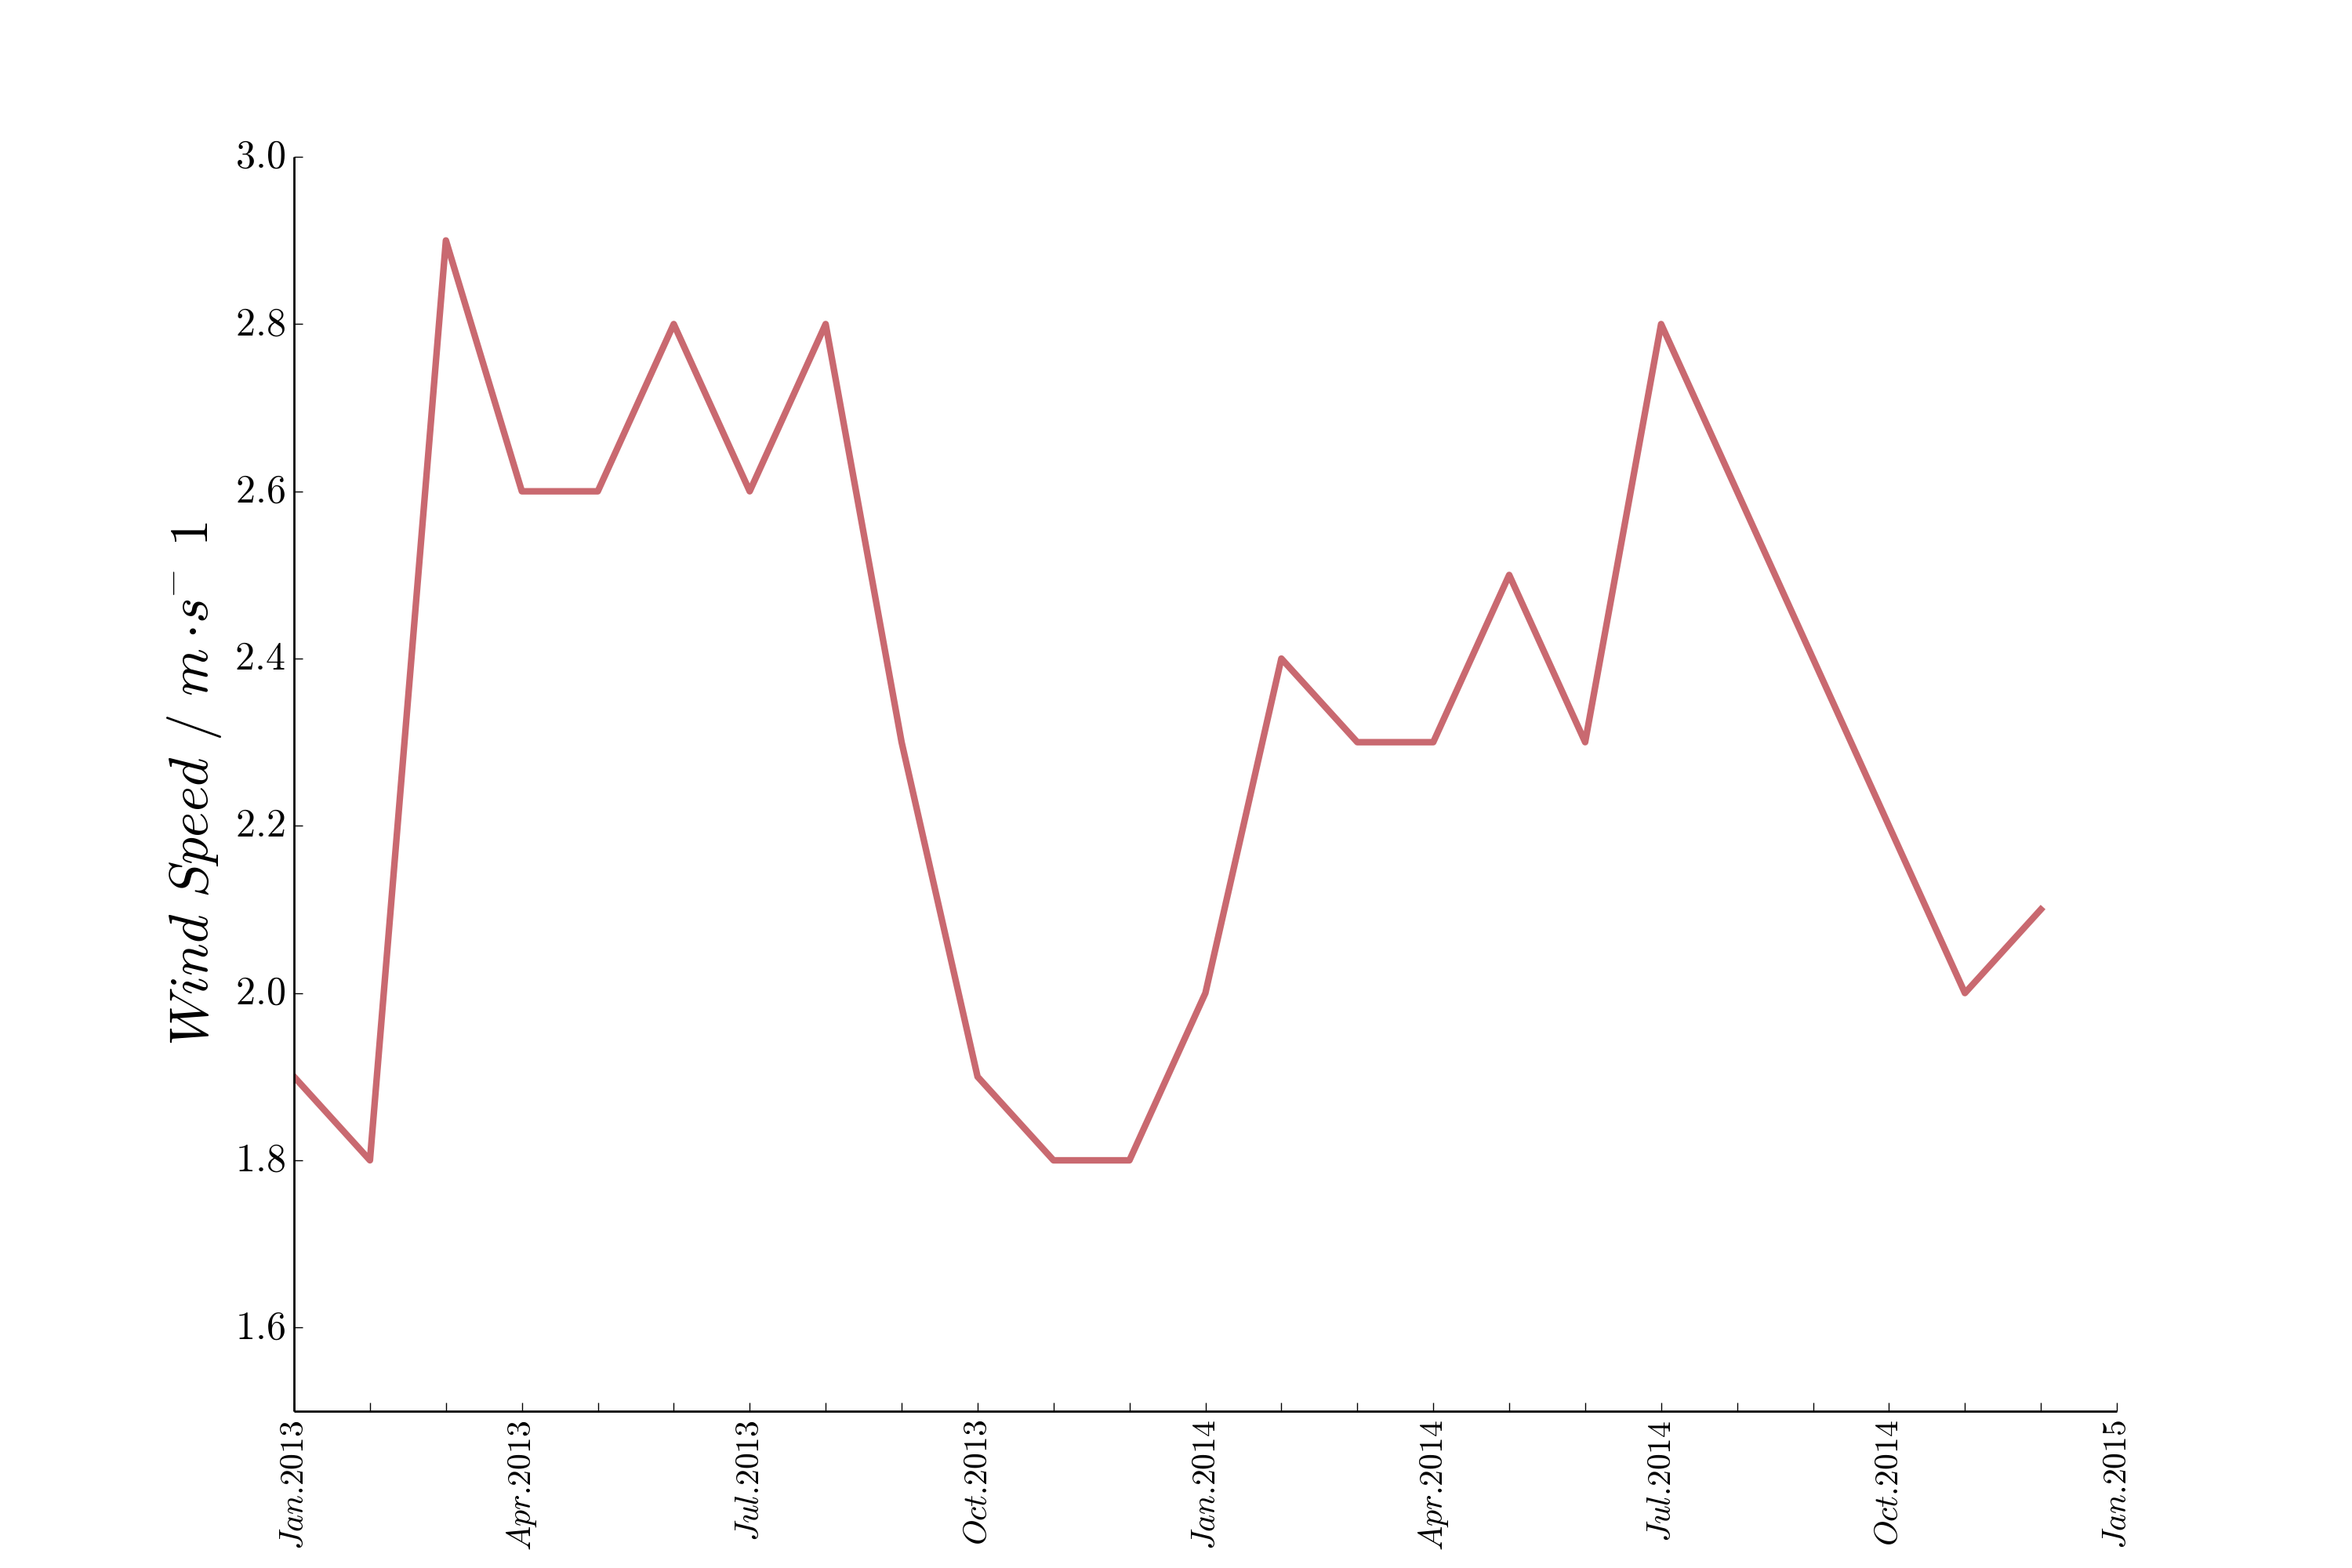
\includegraphics[width=1\textwidth]{./Pic/wind.png}
  %\framebox{Text}
  \caption{Average Wind Speed(2013-2014)}
  \label{fig:wind}
  \end{minipage}
\end{figure}



\begin{itemize}
\item Average Precipitation
\par Precipitation and AQI show a negative correlation trend. The more rain, the better air quality.
\item Average Temperature
\par Temperature and AQI show a negative correlation trend. The higher temperature is high, the better air quality.
\item Average Wind Speed
\par Wind Speed and AQI show a negative correlation trend. The larger the wind, the better air quality.
\end{itemize}



\subsection{Central Heating}
\par Fossil-fuel combustion related winter heating has become a major air quality and public health concern in Xi'an recently. We analyzed the impact of winter heating on air quality index, the result is obviously that the central heating would make striking rise on AQI. The figure as follows.

\begin{figure}[h]%[!hptb] !h意思是忽略美学标准,将照片固定到此位置;不会上下浮动% 支持格式eps, pdf, png, jpg
\centering %使得插入的照片居中显示
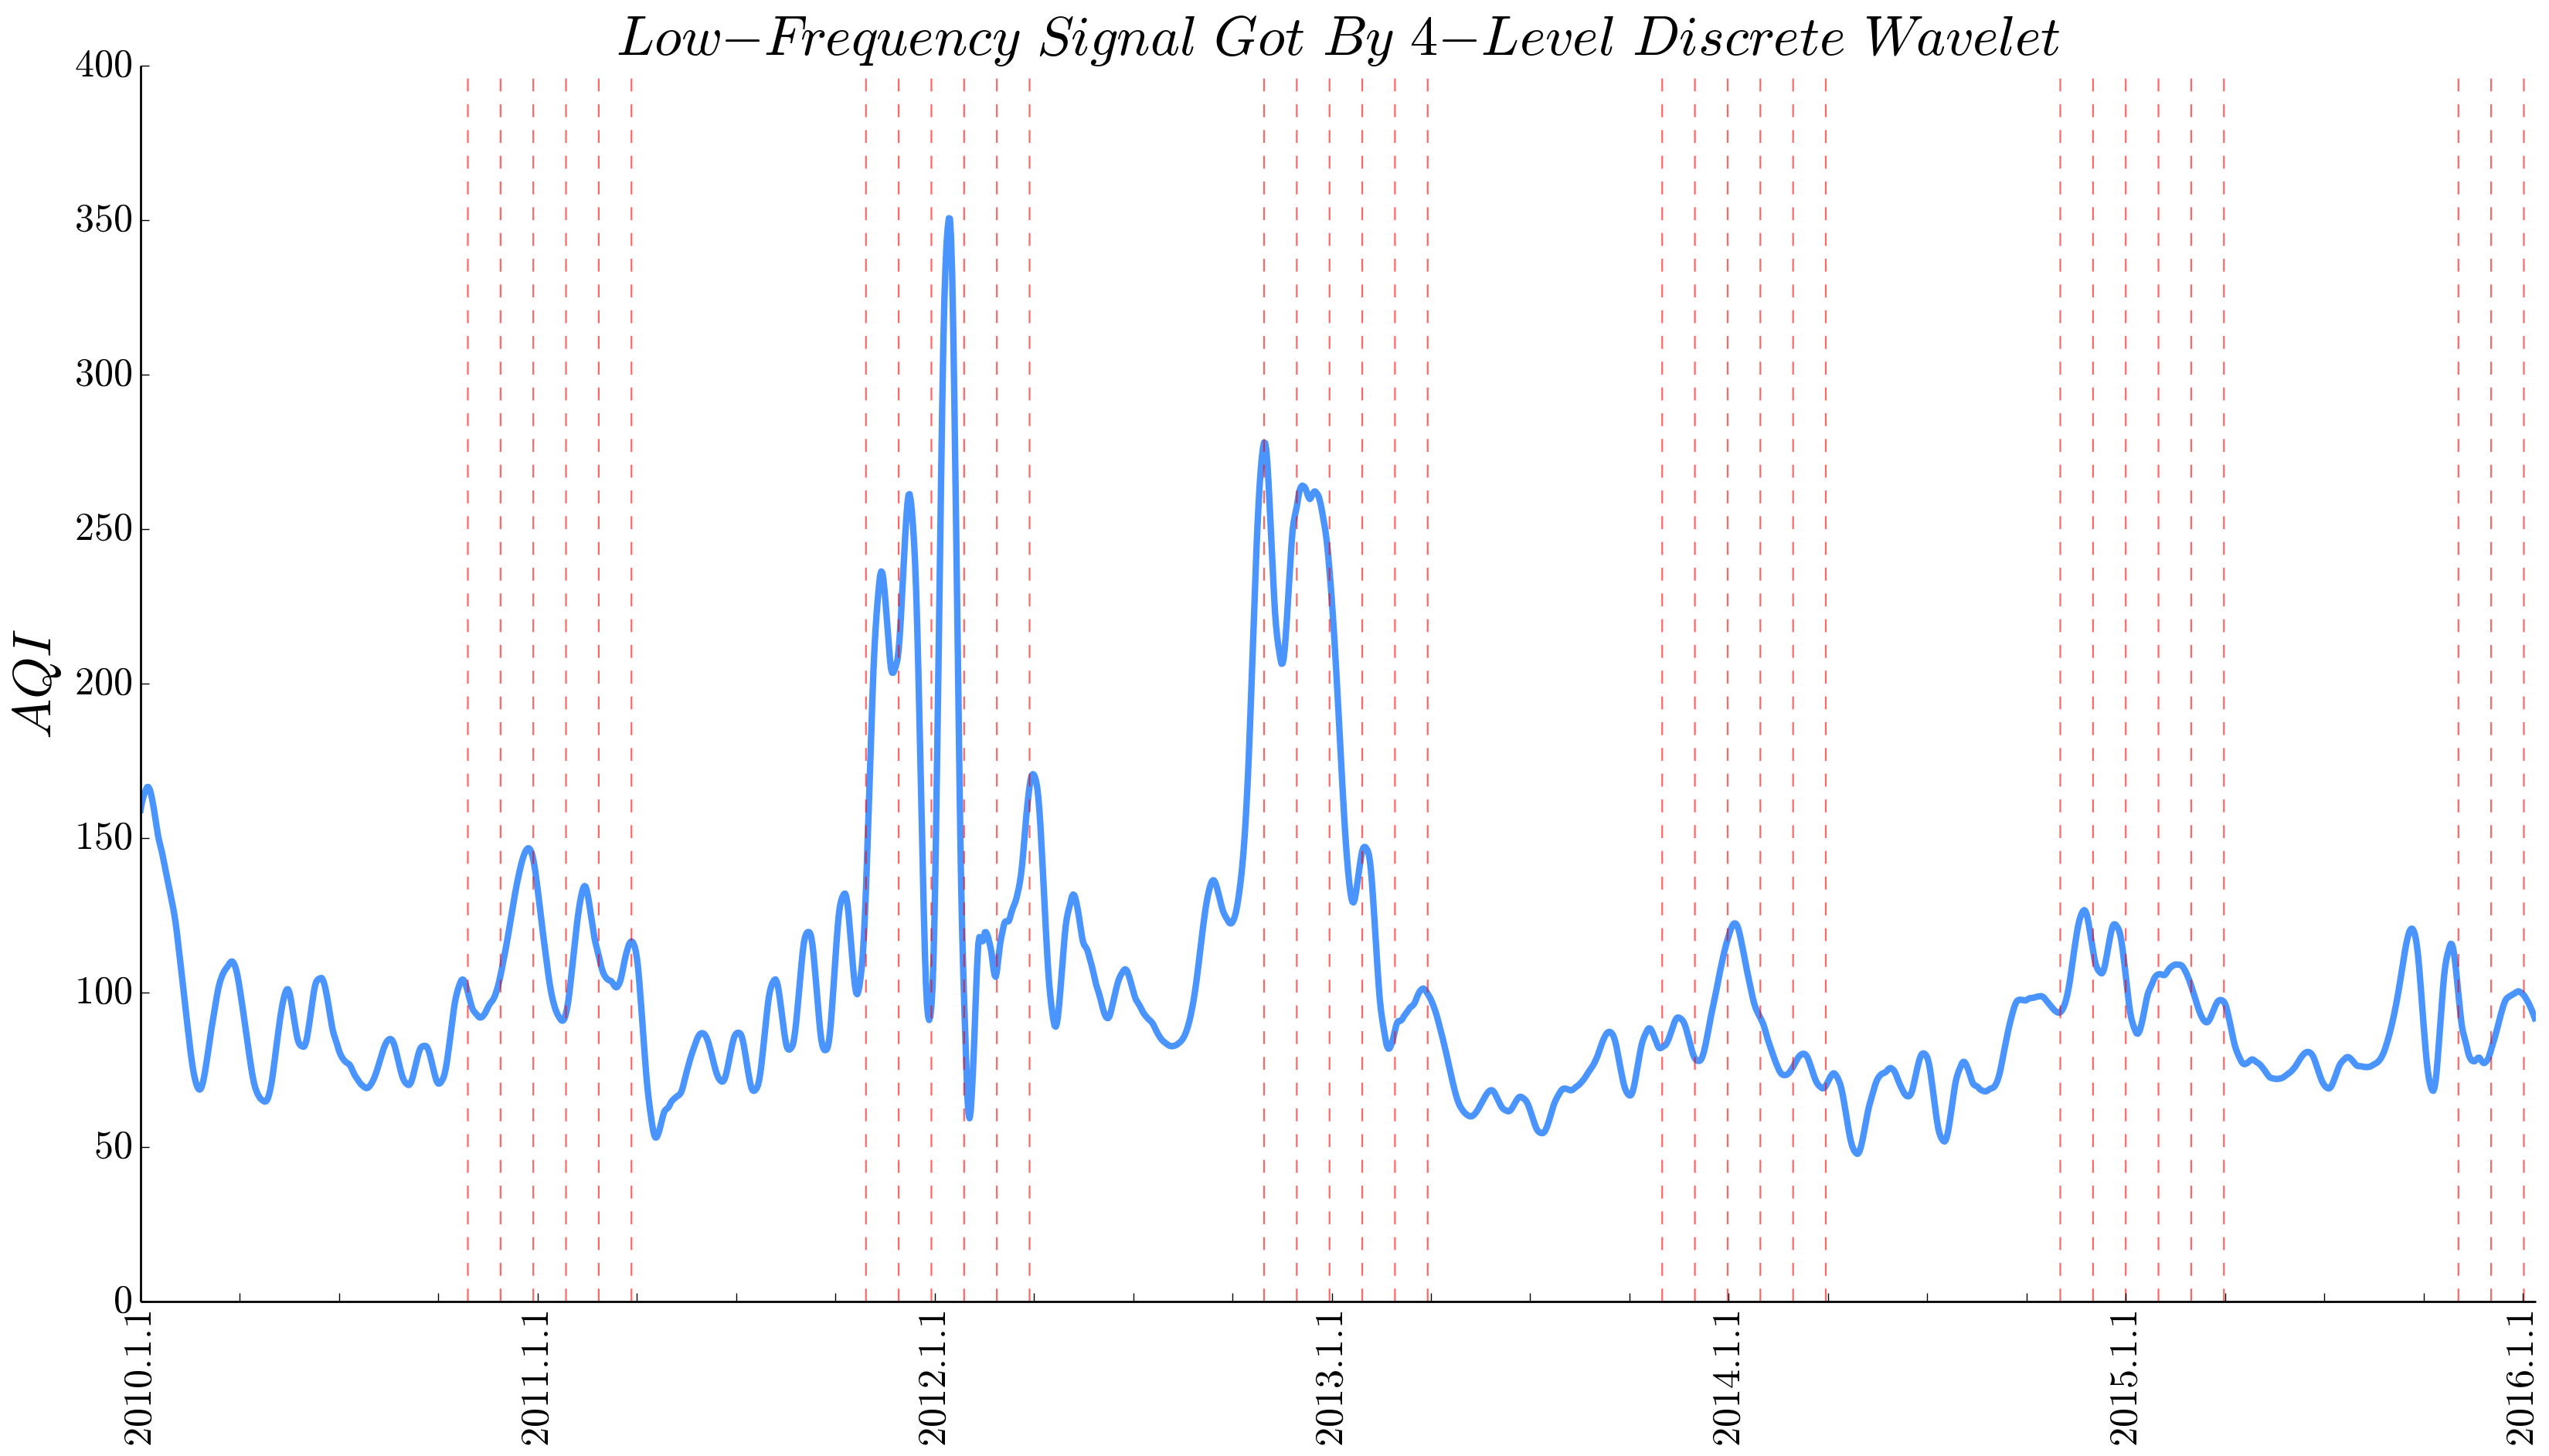
\includegraphics[width=0.50\textwidth]{./Pic/Trslowf.png}
% 图片标题
\caption{the Impact of Central Heating}
\label{fig:Trslowf}       % 给图片一个标签便于交叉引用
\end{figure}

\par The area marked in figure using black lines  represent the center hearting period. From the figure above, our findings suggest that adopting pollution control facilities in power plants and heating stations are needed to improve winter air quality in Xi'an. Furthermore, developing heating systems supplied by renewable energy may be another sustainable solution for air quality improvement.

\section{Strengths and Weaknesses}

\subsection{Strengths}
\par Our model effectively achieves all of the goals we set initially. It is fast and can handle large quantities data of air quality, but also have the flexibility we desired.Though we did not test all kinds of impact factors, we showed that our model optimizes state districts for any of a number of variables.Our model can evaluate all kinds of AQI data from past to the present, it has wide range of application and good time applicability.As well, our method is robust.

\subsection{Weaknesses}
\par Weakness of the model included assumptions made for simplicity that likely do not hold. And some special data can't be found, such as the data of gross industrial production. And it makes that we have to do some proper assumption before the solution of our models. A more abundant data resource can guarantee a better result in our models.

\section{Smog Suggestion Letter in Xi'an}
\textbf{\Large{\emph{Long for Blue Sky ---- a letter from Fresh Air Guardian team to mayor}}}
\par   ~~~~~~~~~~
\textrm{\\}
\leftline{Dear Mayor,}
\par Getting a breath of fresh air isn't as easy as it used to be. We've loaded the atmosphere with all kinds of pollutants that have triggered a number of serious atmospheric ills. The atmosphere is, in effect, talking back. It's warning us that it can't sustain more of our abuse without causing harm.

\par Pollution is the one of the biggest problem affecting the people in Xi'an. Even though the government has established strict law to control this issue, air pollution is still inevitable to some extent. However, some of the facts that why does the air pollution is so hazardous still not be discoverd.Our team has referred to some data, and make our conclusion as follows.
\par There are many kinds of pollution. Air, soil, water and sound pollution are some. Meanwhile, for aie pollution, it is made up of many sources of pollution, such as $NO_2$, $SO_2$, $CO$~and so on. It is difficult to say which one is more risky than the other because all of them are dangerous and equally damage people's health.
\par Through analysing the air condition in Xi'an by our team, according to the pie chart below, we find that the central heating, vehicles, and the factories are the main influencing factors, which accounted for ~89.6\%.

\begin{figure}[h]%[!hptb] !h意思是忽略美学标准,将照片固定到此位置;不会上下浮动% 支持格式eps, pdf, png, jpg
\centering %使得插入的照片居中显示
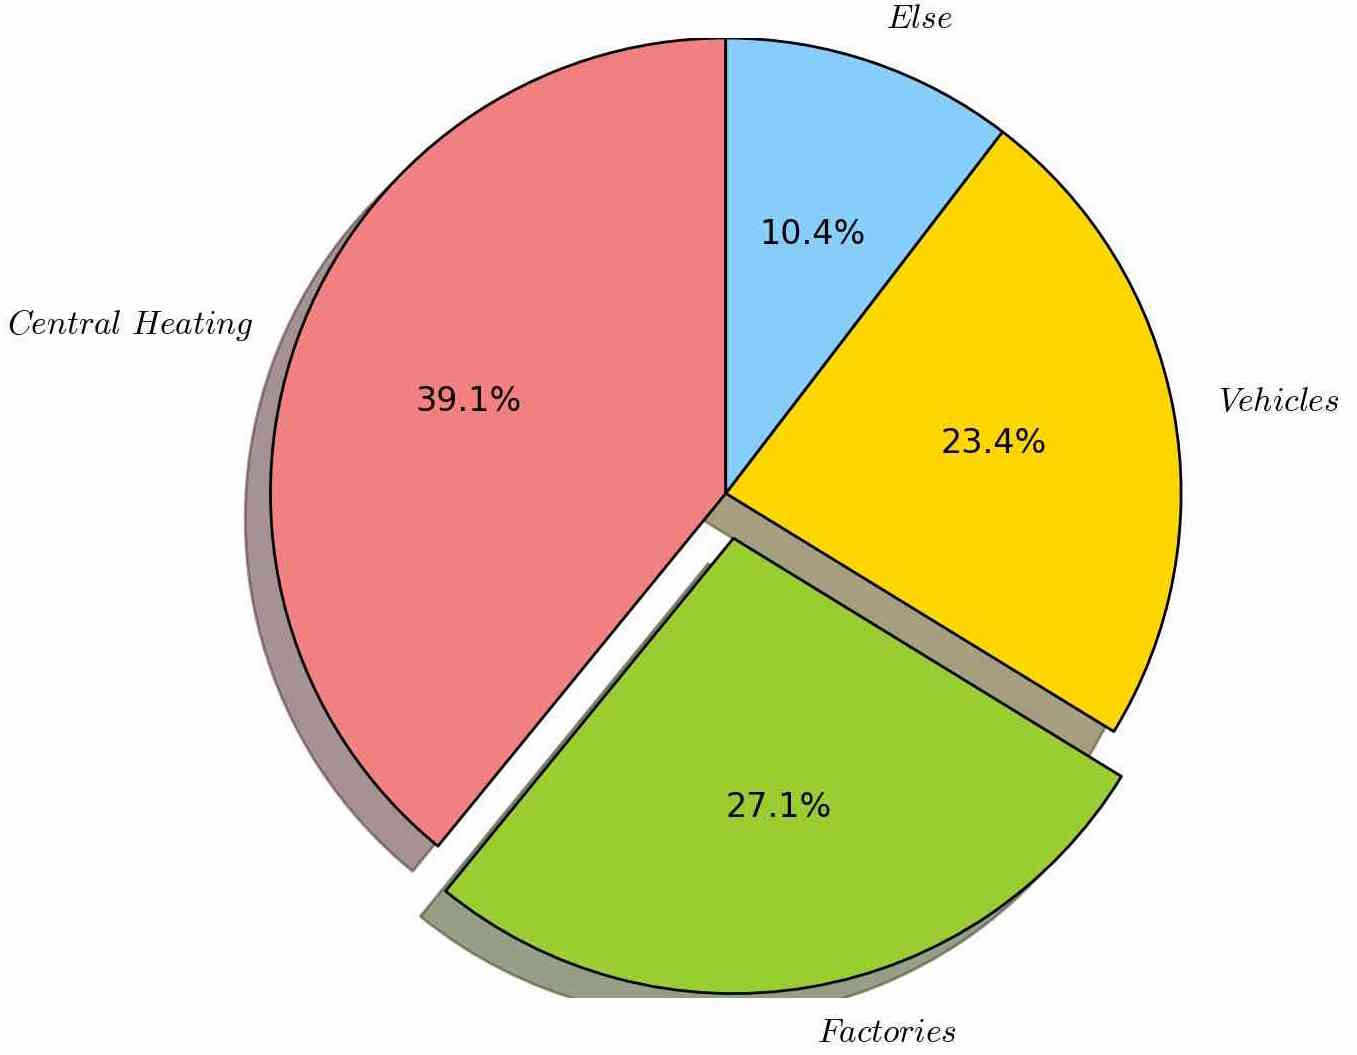
\includegraphics[width=0.50\textwidth]{./Pic/pie.jpg}
% 图片标题
\caption{The Influence of Different Factors on Air Pollution}
\label{fig:pie}       % 给图片一个标签便于交叉引用
\end{figure}


\par According to the finding above, we would like to suggest some measures for controlling the growing air pollution in our city.

\par First of all, all heavy vehicles (HCVs) should be banned from entering the city and only light commercial vehicles, such as tempos should carry the goods to the heart of the city. The transport buses plying within the city should be replaced by electric vans and trolleys to ferry commuters within the city. 

\par Secondly, all factories should be shifted to far-flung areas of the city. These steps along with the working of the complete Metro system will help in controlling the growing air pollution in the city. Unless such and other similar steps are taken immediately, the problem of air pollution will certainly assume serious proportions. 

\par The last but not the least, our government ought to consider forward-looking regulations to allow for carpooling and ride-sharing in the city. This will help de-congest roads, improve commute times, and take cars off the road. This would be achieved by Uber or Didi Dache. Meanwhile, encourage using the green energy. Green energy that produces no greenhouse gas emissions from fossil fuels and reduces some types of air pollution.
\par Our government should follow people's wishes to control air pollution even at the cost of less GDP and revenue. This may not make your term achievements dazzling, but what's more important than citizens' health and safety?

\par I hope the concerned authorities will pay prompt attention to this growing menace and initiate action.
\par 
\rightline{Yours truly,}
\rightline{Fresh Air Guardian team}



%以下是参考文献
\phantomsection%生成该页的链接
\addcontentsline{toc}{section}{\refname}
\begin{thebibliography}{}
%
% 使用指令\bibitem 构造一条参考文献.
% 具体构造方式,参考以下参考文献格式说明以及示例
% 应尽可能使用英文格式
%
\bibitem{1} D.~E. KNUTH   The \TeX{}book  the American
Mathematical Society and Addison-Wesley
Publishing Company  ,  1984-1986.
\bibitem{2}Lamport ,  Leslie ,   \LaTeX{}: `` A Document Preparation System '' , 
Addison-Wesley Publishing Company ,  1986.
\bibitem{RA}
Ministry of environmental protection of the people's Republic of China, Technical Regulation on Ambient Air Quality Index (on trial). \url{http://kjs.mep.gov.cn/hjbhbz/bzwb/dqhjbh/jcgfffbz/201203/t20120302_224166.htm}. 2012
\bibitem{RB}
Xi'an environmental monitoring station, Air quality historical data. \url{http://www.xianemc.gov.cn/sxmpcp_qt.asp?lb=%D6%CA%C1%BF%C8%D5%B1%A8}. 2015
\bibitem{RC}
SPSS China, Homepage. \url{http://www.spss.com.cn/}. 2016

\bibitem{RefJ}
Pope CA, Dockery DW (2006) Health effects of fine particulate air pollution: Lines that connect. Journal of the Air \& Waste Management Association. pp. 709-742.
\bibitem{RefB}
Cao JJ, Lee SC, Chow JC, Watson JG, Ho KF,et al. (2007) Spatial and seasonal distributions of carbonaceous aerosols over China. Journal of Geophysical Research-Atmospheres.
\bibitem{RefC}
Zhao PS, Dong F, He D, Zhao XJ, Zhang XL, et al. (2013) Characteristics of concentrations and chemical compositions for PM2.5 in the region of Beijing, Tianjin, and Hebei,China. Atmospheric Chemistry and Physics 13: 4631-4644. doi:10.5194/acp-13-4631-2013
\bibitem{RefD}
Anonymous (2011) China Electric Power Yearbook China: China Electric Power Press. doi: 10.1080/17437199.2011.587961. pmid:25473706
\bibitem{RefE}
Song Y, Zhang Y, Xie S, Zeng L, Zheng M, et al. (2006) Source apportionment of PM2.5 in Beijing by positive matrix factorization. Atmospheric Environment 40: 1526-1537. doi: 10.1016/j.atmosenv.2005.10.039


% etc
\end{thebibliography}

\begin{appendices}
% 添加多目录
% \include{Appendix1}
% This is Appendix1
% \include{Appendix2}
% This is Appendix2
\section{First appendix}



\begin{longtable}{ccccccc}
 &&&Original Data&&&\\
 \hline
Time  & $SO_2(mg/m^3 $)&$NO_2(mg/m^3) $& $PM_10(mg/m^3) $& $CO (mg/m^3) $&$O_3(8/h~ug/m^3)$& $PM_2.5(ug/m^3)$ \\
\hline
\endhead
% header ------------------------
Jan-13 & 0.118 & 0.08  & 0.298 & 3.628 & 40    & 206 \\
    Feb-13 & 0.079 & 0.061 & 0.263 & 3.641 & 54    & 203 \\
    Mar-13 & 0.055 & 0.072 & 0.345 & 2.942 & 68    & 122 \\
    Apr-13 & 0.031 & 0.061 & 0.19  & 2.2   & 81    & 82 \\
    May-13 & 0.021 & 0.048 & 0.122 & 1.3   & 86    & 57 \\
    Jun-13 & 0.017 & 0.036 & 0.09  & 1.342 & 95    & 42 \\
    Jul-13 & 0.015 & 0.036 & 0.094 & 1.4   & 103   & 52 \\
    Aug-13 & 0.021 & 0.039 & 0.115 & 1.1   & 116   & 59 \\
    Sep-13 & 0.029 & 0.053 & 0.136 & 1.563 & 93    & 79 \\
    Oct-13 & 0.036 & 0.07  & 0.199 & 2    & 69    & 116 \\
    Nov-13 & 0.048 & 0.054 & 0.139 & 1.8  & 27    & 66 \\
    Dec-13 & 0.085 & 0.076 & 0.287 & 3.2  & 26    & 182 \\
    Jan-14 & 0.093 & 0.079 & 0.247 & 2.9  & 29    & 146 \\
    Feb-14 & 0.066 & 0.056 & 0.24  & 2.4  & 34    & 171 \\
    Mar-14 & 0.036 & 0.051 & 0.19  & 2.2  & 52    & 84 \\
    Apr-14 & 0.016 & 0.044 & 0.149 & 1.7  & 66    & 63 \\
    May-14 & 0.015 & 0.032 & 0.144 & 1.5  & 80    & 55 \\
    Jun-14 & 0.013 & 0.034 & 0.096 & 1.4  & 108   & 46 \\
    Jul-14 & 0.011 & 0.035 & 0.086 & 1   & 130  & 35 \\
    Aug-14 & 0.012 & 0.041 & 0.093 & 1.2  & 106   & 44 \\
    Sep-14 & 0.011 & 0.041 & 0.075 & 1.3  & 66    & 40 \\
    Oct-14 & 0.021 & 0.051 & 0.15  & 1.5  & 54    & 78 \\
    Nov-14 & 0.039 & 0.051 & 0.151 & 1.9  & 29    & 84 \\
    Dec-14 & 0.055 & 0.051 & 0.148 & 2   & 27    & 67 \\
\end{longtable}





\section{Second appendix}

\begin{longtable}{ccccccccc}
 &&Processed Data&&&&&&\\
 \hline
Time  & Location & SO2   & NO2   & PM10  & CO    & O3    & PM2.5 & AQI \\
\hline
\endhead
% header ------------------------
2016-1-1 & High Voltage Switch Factory & 59    & 112   & 115   & 27    & 18    & 137   & 137 \\
    2015-12-31 & High Voltage Switch Factory & 58    & 114   & 159   & 65    & 42    & 180   & 180 \\
    2015-12-30 & High Voltage Switch Factory & 39    & 50    & 97    & 45    & 33    & 102   & 102 \\
    2015-12-29 & High Voltage Switch Factory & 46    & 114   & 138   & 68    & 19    & 175   & 175 \\
    2015-12-28 & High Voltage Switch Factory & 40    & 97    & 141   & 40    & 6     & 198   & 198 \\
    2015-12-27 & High Voltage Switch Factory & 48    & 85    & 100   & 35    & 17    & 145   & 145 \\
    2015-12-26 & High Voltage Switch Factory & 47    & 68    & 74    & 36    & 22    & 87    & 87 \\
    2015-12-25 & High Voltage Switch Factory & 42    & 68    & 70    & 36    & 19    & 74    & 74 \\
    2015-12-24 & High Voltage Switch Factory & 34    & 62    & 111   & 29    & 26    & 124   & 124 \\
    2015-12-23 & High Voltage Switch Factory & 68    & 108   & 216   & 60    & 6     & 272   & 272 \\
    2015-12-22 & High Voltage Switch Factory & 59    & 101   & 128   & 49    & 8     & 193   & 193 \\
    2015-12-21 & High Voltage Switch Factory & 54    & 104   & 153   & 70    & 6     & 217   & 217 \\
    2015-12-20 & High Voltage Switch Factory & 48    & 104   & 146   & 56    & 8     & 203   & 203 \\
    2015-12-19 & High Voltage Switch Factory & 53    & 80    & 116   & 37    & 11    & 155   & 155 \\
    2015-12-18 & High Voltage Switch Factory & 29    & 65    & 86    & 25    & 18    & 98    & 98 \\
    2015-12-17 & High Voltage Switch Factory & 22    & 73    & 81    & 31    & 19    & 80    & 81 \\
    2015-12-16 & High Voltage Switch Factory & 12    & 73    & 61    & 24    & 28    & 38    & 73 \\
    2015-12-15 & High Voltage Switch Factory & 15    & 74    & 82    & 26    & 26    & 80    & 82 \\
    2015-12-14 & High Voltage Switch Factory & 19    & 98    & 75    & 39    & 14    & 77    & 98 \\
    2015-12-13 & High Voltage Switch Factory & 16    & 35    & 65    & 49    & 13    & 65    & 65 \\
    2015-12-12 & High Voltage Switch Factory & 22    & 22    & 90    & 50    & 16    & 105   & 105 \\
    2015-12-11 & High Voltage Switch Factory & 34    & 17    & 113   & 50    & 21    & 137   & 137 \\
    2015-12-10 & High Voltage Switch Factory & 29    & 29    & 115   & 50    & 8     & 118   & 118 \\
    2015-12-9 & High Voltage Switch Factory & 51    & 40    & 155   & 53    & 6     & 158   & 158 \\
    2015-12-8 & High Voltage Switch Factory & 39    & 45    & 145   & 50    & 6     & 155   & 155 \\
    2015-12-7 & High Voltage Switch Factory & 51    & 101   & 154   & 56    & 10    & 158   & 158 \\
    2015-12-6 & High Voltage Switch Factory & 60    & 93    & 149   & 50    & 8     & 150   & 150 \\
    2015-12-5 & High Voltage Switch Factory & 60    & 110   & 120   & 50    & 9     & 105   & 120 \\
    2015-12-4 & High Voltage Switch Factory & 45    & 102   & 81    & 49    & 22    & 59    & 102 \\
    2015-12-3 & High Voltage Switch Factory & 31    & 90    & 80    & 45    & 22    & 49    & 90 \\
    2015-12-2 & High Voltage Switch Factory & 23    & 68    & 116   & 43    & 26    & 50    & 116 \\
    2015-12-1 & High Voltage Switch Factory & 34    & 110   & 157   & 56    & 12    & 165   & 165 \\
    2015-11-30 & High Voltage Switch Factory & 37    & 124   & 365   & 71    & 6     & 325   & 365 \\
    2015-11-29 & High Voltage Switch Factory & 40    & 110   & 223   & 62    & 11    & 266   & 266 \\
    2015-11-28 & High Voltage Switch Factory & 40    & 106   & 181   & 58    & 7     & 208   & 208 \\
    2015-11-27 & High Voltage Switch Factory & 45    & 98    & 106   & 42    & 18    & 82    & 106 \\
    2015-11-26 & High Voltage Switch Factory & 32    & 82    & 58    & 36    & 16    & 32    & 82 \\
    2015-11-25 & High Voltage Switch Factory & 17    & 68    & 55    & 37    & 24    & 35    & 68 \\
    2015-11-24 & High Voltage Switch Factory & 5     & 69    & 34    & 39    & 12    & 23    & 69 \\
    2015-11-23 & High Voltage Switch Factory & 11    & 65    & 42    & 39    & 6     & 30    & 65 \\

\end{longtable}



\end{appendices}


\end{document}
